% !TeX program = pdfLaTeX
\documentclass[authoryear, review]{elsarticle} % for elsevier submission
\usepackage{amsmath}
\usepackage{graphicx,psfrag,epsf}
\usepackage{enumerate}
\usepackage{natbib}
\usepackage{textcomp}
\usepackage[hyphens]{url} % not crucial - just used below for the URL
\usepackage{hyperref}
\usepackage{listings} 
\usepackage{booktabs}
\usepackage{float}
\usepackage{threeparttable}
\usepackage{threeparttablex}
%\usepackage[onehalfspacing]{setspace}
\usepackage[usenames,dvipsnames]{color}    
\usepackage[font=small, font+=singlespacing,labelfont=bf]{caption}
\usepackage[pagewise]{lineno}

\lstset{ 
  language=R,                     % the language of the code
  basicstyle=\scriptsize\ttfamily,      % the size of the fonts that are used for the code
  numbers=left,                   % where to put the line-numbers
  numberstyle=\scriptsize\color{Blue},  % the style that is used for the line-numbers
  stepnumber=1,                   % the step between two line-numbers. If it is 1, each line
                                  % will be numbered
  numbersep=5pt,                  % how far the line-numbers are from the code
  backgroundcolor=\color{white},  % choose the background color. You must add \usepackage{color}
  showspaces=false,               % show spaces adding particular underscores
  showstringspaces=false,         % underline spaces within strings
  showtabs=false,                 % show tabs within strings adding particular underscores
  frame=single,                   % adds a frame around the code
  rulecolor=\color{black},        % if not set, the frame-color may be changed on line-breaks within not-black text (e.g. commens (green here))
  tabsize=2,                      % sets default tabsize to 2 spaces
  captionpos=b,                   % sets the caption-position to bottom
  breaklines=true,                % sets automatic line breaking
  breakatwhitespace=false,        % sets if automatic breaks should only happen at whitespace
  keywordstyle=\color{RoyalBlue},      % keyword style
  commentstyle=\color{YellowGreen},   % comment style
  stringstyle=\color{ForestGreen}      % string literal style
}
 
\providecommand{\tightlist}{%
  \setlength{\itemsep}{0pt}\setlength{\parskip}{0pt}}

%\pdfminorversion=4
% NOTE: To produce blinded version, replace "0" with "1" below.
%\newcommand{\blind}{0}

% DON'T change margins - should be 1 inch all around.
% \addtolength{\oddsidemargin}{-.5in}%
% \addtolength{\evensidemargin}{-.5in}%
% \addtolength{\textwidth}{1in}%
% \addtolength{\textheight}{1.3in}%
% \addtolength{\topmargin}{-.8in}%

%% load any required packages here

\makeatletter
\newcommand*{\centerfloat}{%
  \parindent \z@
  \leftskip \z@ \@plus 1fil \@minus \textwidth
  \rightskip\leftskip
  \parfillskip \z@skip}
\makeatother

\begin{document}

%\def\spacingset#1{\renewcommand{\baselinestretch}%
%{#1}\small\normalsize} \spacingset{1}

%%%%%%%%%%%%%%%%%%%%%%%%%%%%%%%%%%%%%%%%%%%%%%%%%%%%%%%%%%%%%%%%%%%%%%%%%%%%%%

\title{Testing for Complementarities between Accounting Practices}

\author[uwa]{Stijn Masschelein \corref{thanks}}
\author[mu]{Frank Moers \corref{thanks}}

\address[uwa]{University of Western Australia Business School, Department of Accounting and Finance, 35 Stirling Highway, Crawley 6009, Australia.}
\address[mu]{Maastricht University School of Business and Economics, Department of Accounting \& Information Management, P.O. Box 616, 6200 MD Maastricht, The Netherlands.}

\cortext[thanks]{The authors are grateful for comments by two anonymous reviewers, David Bedford, seminar participants at Leuven University, Australian National University, the University of Technology Sydney, the University of New South Wales, the University of Western Australia, the Vienna University of Economics and Business, the 2018 AFAANZ conference, and the 2018 AOS conference on Management Control as System or Package in Maastricht.}
% \author{
% Stijn Masschelein \thanks{The authors are grateful for comments by two anonymous reviewers, David Bedford, seminar participants at Leuven University, Australian National University, the University of Technology Sydney, the University of New South Wales, the University of Western Australia, the Vienna University of Economics and Business, the 2018 AFAANZ conference, and the 2018 AOS conference on Management Control as System or Package in Maastricht.} \\
% University of Western Australia Business School\\
%  and \\     Frank Moers \\
% Maastricht University School of Business and Economics\\
%   }

\begin{abstract}
Following the theoretical innovations of complementarity theory, management control studies have investigated interdependencies between different management control practices. In this paper, we compare the two dominant statistical specifications to test for the presence of an interdependency. We show theoretically how the power of the demand and the performance specification varies with the level of optimality in the sample and how those specifications are vulnerable to correlated omitted variable bias. Our simulation results reveal that the demand specification is more robust to variations in optimality and correlated omitted variables than the performance specification. We use these results to formulate recommendations for future research into management control interdependencies.
\end{abstract}

\maketitle

\noindent%
{\it Keywords:} Complementarity Theory, Management Control, Statistical Methods
\vfill

\newpage

%\spacingset{1.15}

\section{Introduction}\label{introduction}

The management accounting literature has investigated the fit between accounting practices and the firms' environment \citep{chenhall_management_2003, otley_contingency_2016}, as well as the firms' choices of interdependent practices such as delegation and incentives \citep{bouwens_assessing_2007, indjejikian_accounting_2012, moers_performance_2006}, or the levers of control \citep{simons_levers_1994, simons_performance_2000, widener_empirical_2007}. The interdependencies between different practices are the reason a collection of practices form an accounting system  \citep{grabner_management_2013,milgrom_complementarities_1995}. When two practices positively reinforce or complement each other, the firm benefits from using them together, as a system. When two practices negatively reinforce each other, they act as substitutes. In this paper, we compare the two most common specifications in the empirical literature to test whether practices are complements (or substitutes), i.e., the performance specification and the demand specification \citep{grabner_management_2013}, and examine the vulnerability of these specifications to their underlying assumptions. 

The performance specification tests whether the interaction between two practices is postively correlated with performance \citep{athey_empirical_1998, carree_note_2011, grabner_management_2013, hofmann_organizational_2017}. For instance, the interaction between delegation and accounting based incentives is positively related to business unit performance. The performance specification assumes that there are a "sufficient number" of firms that deviate from the optimal level for the practices which allows researchers to detect performance differences between optimal and suboptimal accounting systems. The extreme version of this assumption is that all firms make random choices. The demand specification on the other hand tests whether two practices are positively correlated with each other after controlling for environmental factors \citep{arora_testing_1996, grabner_management_2013, johansson_testing_2018, hofmann_organizational_2017}.  For instance, delegation and accounting based incentives are correlated after controlling for environmental factors. The demand specification assumes that there are a "sufficient number" of firms that simultaneously choose the optimal level of the practices taking into account the interdependency and the firm's environment. The extreme version of this assumption is that all firms make optimal choices.

In observational samples neither the assumption of completely randomly chosen practices nor the assumption of completely optimal choices will hold \citep{brynjolfsson_complementarity_2013}. While an individual decision is either optimal or not, a non-optimal decision can be closer or further from the optimal level. As a result, a sample of those individual decisions can exhibit different levels of optimality where higher levels of optimality imply more observations that are close to the optimal decision. The methodology literature has treated the assumption about the level of optimality in a sample as an untestable assumption and recommends that researchers argue whether their chosen specification is appropriate for their research setting. The demand specification is often seen as more appropriate than the performance specification when one decision maker has designed the entire accounting system, when the optimal design is not too complicated, and when the decision maker has had sufficient time and incentives to choose the optimal system \citep{grabner_management_2013, hofmann_organizational_2017, carree_note_2011, johansson_testing_2018}.  The performance specification is often deemed more appropriate when it involves relatively new practices and technologies that require experimentation \citep{carree_note_2011, bedford_management_2016}. While these recommendations are intuitive, their empirical validity is not clear. That is, it is not clear how vulnerable each specification is to deviations from its underlying assumption of (lack of) optimality and whether this vulnerability differs between the two specifications. The key question we address in this paper is whether the typical arguments for choosing a specification are necessary and/or sufficient.

In addressing this question, we first show how the demand and performance specification arise from the same underlying and unobserved objective function. The objective function formalises the performance effects of management accounting practices as well as how those performance effects depend on other practices and contingency factors. As a result, the objective function captures the main insight of complementarity theory \citep{milgrom_complementarities_1995,grabner_management_2013} and contingency theory \citep{chenhall_management_2003,otley_contingency_2016} and is thus the theoretical foundation for a hypothesis test regarding interdependencies. We then show the statistical problems that arise with the demand and performance specification when the assumptions underlying these specifications are not satisfied. First, the demand specification has more power to detect an interdependency when management control practices are closer to optimal while the performance specification is more likely to detect an interdependency when the control practices are further from optimal. But again, how close to or how far from optimal the practices need to be to have sufficient power is an open question. Second, while the correlated omitted variable problem is widely recognised for the demand specification \citep{grabner_management_2013, arora_testing_1996, hofmann_organizational_2017}, it is largely ignored \citep{grabner_management_2013, hofmann_organizational_2017} or thought of as non-existing for the performance specification \citep{carree_note_2011}. We show that both specifications are vulnerable to the same omitted variable bias when they do not appropriately control for a contingency factor that affects both practices. When all relevant practices and contingency factors are observed, this bias can be easily addressed, although the most commonly used variant of the performance specification unfortunately does not address the bias. However, when not all contingency factors are observed, it is an open question whether the two specifications are equally vulnerable to correlated omitted variables.

To investigate the robustness of both specifications to variations in the level of optimality, we use a simulation approach. In doing this, we focus on Type I errors (rejection of a true null hypothesis of no complementarity) and power (or Type II errors, i.e., failure to reject a false null hypothesis of no complementarity). The results show that the demand specification has appropriate Type I error rates while maintaining power to detect a real complementary effect, even at low levels of optimality. In contrast, the theoretically derived performance specification suffers from elevated Type I error rates at all levels of optimality and loses power to detect true interdependencies at higher levels of optimality. In addition, the performance specification as it is typically implemented in the literature is biased when the practices are contingent on the same environmental factor. Finally, in contrast to common assumptions, even in the presence of correlated omitted variables, the demand specification fares better than the performance specification.

This study contributes to the literature by providing three recommendations for studies that test for interdependencies between management control practices. First of all, the demand specification should generally be preferred over the performance specification in an observational sample of firms. While researchers are typically recommended to argue whether their chosen specification is appropriate for their research setting, our findings indicate that the use of the performance specification needs to be especially well-substantiated. Even when performance data is available, it is still advisable to report the demand functions before reporting the performance specification \citep{aral_three-way_2012, cassiman_search_2006}. Second, when theory and prior research indicate that the practices are contingent on environmental factors, studies should appropriately control for these factors. Because the management control literature has a rich history of studying contingency effects, we believe most management control settings will warrant appropriate controls for contingency factors. Importantly, these controls are as relevant for the performance specification as they are for the demand specification. In the demand specification, controlling for contingency factors means including the contingency variables as separate independent variables. In the performance specification, controlling for contingency effects requires including the interaction of the contingency factors with the management control practices. Of the published studies using the performance specification following \citet{grabner_management_2013}, only \citet{bedford_management_2016, bedford_performance_2019} appropriately control for contingency factors. Third, because the performance specification is vulnerable to Type I errors, we advise to use more robust estimation techniques than ordinary least squares.

The remainder of this paper is structured as follows. First, we derive the demand and performance specifications from a common objective function. Second, we explain and calibrate the simulation approach. Third, we compare the robustness of the different specifications in a simulation study. Fourth, we provide guidance for researchers who estimate interdependencies. Last, we summarise the simulation results and recommendations, and discuss how future research can improve the estimation of interdependencies.

\section{Model and formal analysis}\label{model-and-formal-analysis}

In this section, we present a firm's objective function to model the essential elements of both complementarity theory and contingency theory. According to complementarity theory, the performance effect of a management control practice depends on the use of another practice. According to contingency theory, the performance effect of the practice depends on the environment. The theoretical model helps to make explicit the assumptions in the two statistical specifications. We start with the assumption that a firm has to decide on the level of two management accounting practices which both depend on one environmental factor. We represent the levels of the management accounting practices as  $x_1$ and $x_2$ and the level of the environmental factor as $z$. We further assume that performance, $y$, depends on a factor, $\nu$ while the performance effects of each management control practice further depend on a factor $\epsilon_1$ and $\epsilon_2$ respectively. That is, there is variation among firms in the extent to which each management control practice affects performance. $x_1$, $x_2$ and $z$ are observed by the researcher but $\epsilon_1$, $\epsilon_2$, and $\nu$ are not. 

We illustrate the model with an example from the management accounting literature where $z$ stands for environmental uncertainty, one of the most commonly studied environmental factor in the contingency literature. $x_1$ and $x_2$ are two commonly studied management control decisions, the extent to which decisions are delegated to middle level managers (henceforth delegation) and the extent to which accounting measures are used to evaluate and reward performance of the middle level managers (henceforth accounting incentives). Finally, $y$ is the financial performance of the business unit. These four constructs have received considerable attention in both the contingency and the complementarity literature \citep{grabner_management_2013,chenhall_management_2003, otley_contingency_2016}. In the example, we cannot do justice to the rich theories and measurement developed in the literature and therefore the example should only be seen as an illustration of the objective function. In addition, the linear form is a special case, but its simplicity allows us to make our point without loss of generality.

\begin{equation}\label{eq:objective}
y  = \beta_0 + (\beta_{1} + \gamma_1 z + \epsilon_1) x_1 
						+ (\beta_{2} + \gamma_2 z  + \epsilon_2) x_2 
                        + \beta_{12} x_1 x_2 - \frac{1}{2}\delta_1 x^2_1 - \frac{1}{2}\delta_2 x^2_2 + \nu
\end{equation}
The objective function \eqref{eq:objective} shows how profit, $y$, depends on delegation and accounting incentives, $x_1$ and $x_2$, environmental uncertainty $z$ and the unobservable factors. The parameter $\beta_{12}$ represents the complementarity between delegation and accounting incentives (i.e. $\frac{\delta^2 y}{\delta x_1 \delta x_2} = \beta_{12}$, see \citet{grabner_management_2013}). Irrespective of which empirical test will be performed, interdependence implies that $\beta_{12}\neq0$ and this is what needs to be theoretically substantiated. In this paper, we focus on specifications to test the hypothesis that $\beta_{12} \neq 0$.\footnote{Initially, we limit the paper to two-way complementarities for two reasons. First, theory in management control typically does not predict higher order interdependencies (for an exception outside of management accounting see \citet{aral_three-way_2012}). Second, the paper's main focus is on the consequences of deviations from completely optimal and completely random practices for hypothesis tests. The problems we identify apply to more complex hypothesis tests for higher order interdependencies. For simplicity of exposition, we avoid the additional complications of testing for higher order interdependencies \citep{carree_note_2011}. In section \ref{contingent-complementarity}, we consider contingency effects on the interdependencies \citep{grabner_incentive_2014, grabner_cost_2016, matejka_balancing_2017} and in section \ref{robustness-demand}, we investigate an objective function with three practices and two-way interdependencies \citep{indjejikian_accounting_2012}.}
An example of such a test is whether the effectiveness of incentive contracts depends on the level of delegation for managers \citep{moers_performance_2006, indjejikian_accounting_2012}. The parameters $\gamma_1$ and $\gamma_2$ represent the contingency effect of environmental uncertainty, $z$, for delegation, $x_1$, and accounting incentives, $x_2$. For instance, $\gamma_1 > 0$ implies that delegation is more valuable for the firm with higher environmental uncertainty while $\gamma_2 < 0$ implies that accounting incentives are less valuable with higher environmental uncertainty \citep{chenhall_management_2003}. 
$\delta_1$ and $\delta_2$, which we assume to be positive, represent increasing marginal costs to the practices.\footnote{$\delta_{1}$ and $\delta_{2}$ are the second derivatives of the performance effects of the practices. In general, $\mathbf{\delta} > 0$ is a mathematical representation of decreasing marginal returns,  increasing marginal  costs, or a combination of both. For simplicity and in line with the specification in \citet{grabner_management_2013}, we interpret $\mathbf{\delta}$ as the parameter of  increasing marginal costs.} 

The objective function \eqref{eq:objective} formalises management accounting theory. The key assumptions of complementarity theory and contingency theory are captured by the parameters $\beta_{12}$ and $\gamma_1, \gamma_2$ respectively. In order to test for a complementarity between delegation and accounting incentives, we need to make additional assumptions about the statistical model, which we discuss below. The theoretical assumptions discussed above and the statistical assumptions discussed below are the same for both the demand specification and the performance specification.

We assume that $\epsilon_1$ and $\epsilon_2$ and $\nu$ are independent which implies that the model contains all contingency variables and all practices that affect the performance of the two practices $x_1$ and $x_2$. The objective function \eqref{eq:objective} is similar to the the objective function in \citet{kretschmer_competitive_2012} with two exceptions. First, we assume that the values of $x_1$ and $x_2$ are continuous while \citet{kretschmer_competitive_2012} allow for binary practices. We return to the issue of binary practices as an extension to the current model in section \ref{binary-practices} and \ref{robustness-demand}. Second, we assume independence of the unobserved factors. We will relax this assumption, when we introduce the problem of correlated omitted variables further in section \ref{correlated-omitted}.\footnote{\citet{athey_empirical_1998} discuss the implications of relaxing the independence assumption in more detail.}  In the remainder of this section, we will work with the simple objective function with two practices and one environmental factor. 

\subsection{Optimal level of practices} \label{optimal-level-of-practices}

Profit maximising firms try to adopt the optimal level for each practice. As a benchmark, we derive the optimal level for all practices by setting the first derivative of the objective function \eqref{eq:objective} to each practice equal to $0$ and then solve for each practice. This results in:

\begin{equation}\label{eq:optimal}
\begin{aligned}
x_1^* &= \frac{\beta_{1} + \gamma_1 z + \beta_{12} x_2^*  + \epsilon_{1}}{\delta_1 }
		      = \frac{\delta_2 (\beta_{1} + \gamma_1 z + \epsilon_1) 
           					+ \beta_{12} (\beta_{2} + \gamma_2 z + \epsilon_2) }
                            {\delta_1 \delta_2 - \beta_{12}^2} \\
 x_2^* &= \frac{\beta_{2} + \gamma_2 z + \beta_{12} x_1^* + \epsilon_{2}}{\delta_2  }
		      =  \frac{\delta_1 (\beta_{2} + \gamma_2 z + \epsilon_2) 
           					+ \beta_{12} (\beta_{1} + \gamma_1 z + \epsilon_1) }
                            {\delta_1 \delta_2 - \beta_{12}^2} \\
\end{aligned}
\end{equation}
A number of conclusions can be drawn from the optimality conditions \eqref{eq:optimal}. First, in the absence of complementarity ($\beta_{12}=0$), the optimal level of delegation, $x^*_1$ and the optimal level of accounting incentives, $x^*_2$ are still correlated. The contingency effects of environmental uncertainty introduce a relation between the optimal level of delegation, $x^*_1$, the optimal level of accounting incentives, $x^*_2$ and environmental uncertainty, $z$. Second, in the absence of a complementarity ($\beta_{12} = 0$) and after controlling for environmental uncertainty, there is no relation between the optimal level of delegation and accounting incentives, i.e. the conditional correlation, $cor(x^*_1 | z, x^*_2 |z) = 0$.  In contrast, in the presence of a complementarity, $\beta_{12} > 0$, the optimal level of delegation positively correlates with the optimal level of accounting incentives after controlling for $z$ \citep{arora_testing_1996}. 

In what follows, we will refer to the observed correlations between the practices and the environmental variable. We define $r_{12}$, $r_{1z}$, and $r_{2z}$ as the observed sample correlations between delegation, $x_1$, and accounting incentives, $x_2$,  between delegation, $x_1$, and environmental uncertainty, $z$, and between accounting incentives, $x_2$, and environmental uncertainty, $z$, respectively. In samples with higher levels of optimality, the observed correlations are determined by the equations \eqref{eq:optimal}.  In samples where management control practices are randomly chosen, the correlations are $0$. 

Finally, the second order condition for the optimality conditions \eqref{eq:optimal} equals $\delta_1 \delta_2 - \beta_{12}^2 > 0$. The intuition behind this condition is that the increase in marginal costs to delegation and accounting incentives needs to be relatively large so that the interdependency does not dominate the optimal solution. That is, it avoids corner solutions where the optimal use of the management control practices is to use them to their full extent or not at all.\footnote{In the main analysis of this paper, we will assume that the second-order condition holds when the control practices are continuous. In Section 4.4 we relax this assumption.}

\subsection{Performance Specification}

The performance specification estimates the objective function \eqref{eq:objective} directly. In essence, the stochastic form of function \eqref{eq:objective} is a regression equation. With cross-sectional data, the closest approximation to the objective function is the first of the following three regression models.  

\begin{align*}
y &=  \beta^{p1}_0 + (\beta^{p1}_{1} + \gamma_1^{p1} z )x_1 
						+ (\beta_{2}^{p1} + \gamma_2 z ) x_2 
                        + \beta_{12}^{p1} x_1 x_2 
                        + \delta_1^{p1} x^2_1 + \delta_2^{p1} x^2_2 
                        + \alpha^{p1} z
                        + \nu^{p1} \\
 y &=  \beta^{p2}_0 + (\beta^{p2}_{1} + \gamma_1^{p2} z )x_1 
						+ (\beta_{2}^{p2} + \gamma_2 z ) x_2 
                        + \beta_{12}^{p2} x_1 x_2 
                        + \alpha^{p2} z
                        + \nu^{p2} \\
 y &=  \beta^{p3}_0 + \beta^{p3}_{1} x_1 
						+ \beta_{2}^{p3} x_2 
                        + \beta_{12}^{p3} x_1 x_2 
                        + \alpha^{p3} z
                        + \nu^{p3}
\end{align*}
The first specification captures all features of the objective function \eqref{eq:objective} with the exception of the unobservable contingency effects on delegation and accounting incentives, $\epsilon_1$ and $\epsilon_2$. Cross-sectional data does not permit estimating the unobserved heterogeneity. In this specification, \(\beta_{12}^{p1}\) tests for the interdependency between the management accounting practices. We are not aware of any accounting studies using this specification, which we label the \emph{performance 1} specification. 

The second specification, which we label the \emph{performance 2} specification, is the correct specification for binary practices, i.e., when practices are either absent or present. In this case, the quadratic terms, $x_i^2$, automatically drop out of the equation. While investigating continuous practices, \citet{ bedford_management_2016, bedford_performance_2019} follow this specification as they control appropriately for contingency factors and drop the quadratic terms in the specification. The majority of the literature follows the third performance specification, which also drops the controls for the contingency factors or assumes that $\gamma_1 = \gamma_1 = 0$. This specification thus ignores the insights from contingency theory. We call this specification \emph{performance 3}. In the remainder of this section, we explain the potential problems with these three specifications.

\subsubsection{Lack of Power}

All three specifications will suffer form the well known problem that performance is no longer a function of the management practices when firms optimally adopt interdependent practices \citep{grabner_management_2013}. This can be illustrated using objective function \eqref{eq:objective} and the optimality conditions \eqref{eq:optimal}. When we set $x_1 = x_1^*$ and $x_2 = x_2^*$ in the objective function  \eqref{eq:objective}, i.e., the firm makes optimal decisions, we find that profit, $y$, is fully determined by the unknown parameters and environmental uncertainty, $z$, and profit no longer depends on the value of the practices. Thus, \textit{observed} profit is not a function of \textit{observed} delegation and \textit{observed} accounting incentives when all firms adopt the optimal system. With optimal levels of delegation and accounting incentives, business unit profit is only a function of environmental uncertainty and there is no longer information about the practices in the performance variable. This is what economists are referring to when they say that one cannot examine performance effects of choices. The point is not that there are no performance effects of adopting management control practices, but rather that such effects cannot be empirically detected. 

The loss of power of the performance specification depends on the level of optimality in the sample. A higher level of optimality leads to stronger  correlations between the control practices and the contingency factor, and less independent information in the \textit{observed} practices about the \textit{observed} profit. For a performance specification to have sufficient power, there needs to be a sufficient number of firms that do not adopt the optimal level of the practices \citep{bedford_management_2016, carree_note_2011, hofmann_organizational_2017}. However, the literature has not gone beyond this rule of thumb and provides no guidance on how large the deviations from optimality need to be. Our simulation study will provide an answer to this question.

\subsubsection{Correlated Omitted Variable}

In this paper, we identify a second problem with the most popular specification in the literature, \emph{performance 3}, which follows directly from the contingency effects. The specification omits the terms $x_1 z$, $x_2 z$, $x_1^2$, and $x_2^2$. Although a full treatment of the omitted variable bias is beyond the scope of this study, we illustrate the problem for the special case where $x_1$, $x_2$, and $z$ follow a multivariate standard normal distribution. Appendix \ref{appendix-omitted} shows that the bias for omitting $x_1 z$, $x_2 z$, $x_1^2$, and $x_2^2$ in the estimate $\beta^{p3}_{12}$ is proportional to the following components:

\begin{equation}\label{eq:omitted}
\begin{aligned}
\gamma_1 \frac{cov(x_1 x_2, x_1 x_2)}{var(x_1 x_2)} &= 
\gamma_1 \frac{r_{2z} + r_{12} r_{1z}}{1 + r_{12}^2}
&\gamma_2 \frac{cov(x_1 x_2, x_2 z)}{var(x_1 x_2)} &= 
\gamma_2 \frac{r_{1z} + r_{12} r_{2z}}{1 + r_{12}^2}
\\
\delta_1 \frac{cov(x_1 x_2, x_1^2)}{var(x_1 x_2)} &= 
\delta_1 \frac{r_{12}}{1 + r_{12}^2}
&\delta_2 \frac{cov(x_1 x_2, x_2^2)}{var(x_2 x_2)} &= 
\delta_2 \frac{r_{12}}{1 + r_{12}^2}
\end{aligned}
\end{equation}
where $r_{12}$, $r_{1z}$, and $r_{2z}$ are the observed sample correlations, as defined before. Let us assume that there is no interdependency, i.e., $\beta_{12}=0$. The estimate $\beta^{p3}_{12}$ , which equals $\beta_{12} + bias$, is then affected by the four components specified in \eqref{eq:omitted}. $\beta^{p3}_{12}=\beta_{12}=0$ when the observed correlations $r_{12}$, $r_{1z}$, and $r_{2z}$ are all zero, or in other words, when firms just randomly pick their management control practices. However, as explained in the previous section, contingency theory implies that those empirical correlations between delegation, accounting incentives, and environmental uncertainty are different from $0$ when firms are not completely ignorant of the optimal levels. As a result, when environmental uncertainty is not appropriately controlled for, the \emph{performance 3} specification is vulnerable to an omitted variable bias when testing for a complementarity between delegation and accounting incentives. The intuition behind the bias is as follows. If delegation, $x_1$, and environmental uncertainty, $z$, are correlated, the interaction between delegation and accounting incentives, $x_1 x_2$, and the interaction between accounting incentives and environmental uncertainty, $x_2 z$, are also correlated. As a result, when the contingency effect, $x_2 z$, is omitted from the performance specification, the complementarity test, $x_1 x_2$, will be confounded by the contingency effect, even when $\beta_{12}=0$. That is, a Type I error occurs. Note that this problem extends to the \emph{performance 1} and \emph{performance 2} specifications when factors unobservable to the researcher affect both practices, which we will address later.

Because the bias does not require perfectly optimal decisions and follows directly from the contingency effect of environmental uncertainty on delegation ($\gamma_1 \neq 0$) and accounting incentives ($\gamma_2 \neq 0$), this problem cannot be easily ignored in a typical management accounting study. A special case of the omitted variable bias is the omission of the quadratic terms $\delta_1 x_1^2$ and $\delta_2 x_2^2$ in \emph{performance 2}. Omission of these terms will bias the estimate of the $\beta^{p2}_{12}$ with a factor proportional to the correlation between delegation and incentives.

The empirical and methodology literature has focused on this bias in the demand specification (see also section \ref{demand-specification}) but has largely ignored the problem of correlated omitted environmental factors in performance specifications. However, in the above, we showed that the performance specifications suffer from the exact same bias in contrast to what has been argued in the methodology literature \citep{carree_note_2011}. 

\subsection{Demand Specification}\label{demand-specification}

The \emph{demand specification} can take two forms, the regression approach and the conditional correlation approach. The first approach regresses one practice (e.g. delegation) on the other (e.g. accounting incentives) and controls for environmental uncertainty.
\begin{equation*} 
x_1 = \beta_1^d + \beta_{12}^d x_2 
        + \gamma_{1}^d z
        + \epsilon^d
\end{equation*}
The regression specification approximates the optimality condition \eqref{eq:optimal} where \(\beta^d_{12}\) is the parameter that estimates the complementarity effect. An alternative and equivalent approach is to estimate the conditional correlation between delegation and incentives. Prior research has used seemingly unrelated regressions with $x_1$ and $x_2$ as dependent variables or seperate regressions to condition on environmental practices \citep{indjejikian_accounting_2012, matejka_balancing_2017}.\footnote{The equivalence between the regression and the conditional correlation follows from the regression anatomy \citep{angrist2008mostly}. That is, $\beta^d_{12}=\frac{cov(x_1, x_2|z)}{var (x_2|z)}=cor(x_1, x_2|z)\frac{stdev(x_1)}{stdev (x_2|z)}$. The semi-partial correlation is directly related to the partial or conditional correlation: $\sqrt{1 - cor^2(x_1, z)} cor(x_1, x_2|z) = cor(x_1|z, x_2|z)$
Thus, $\beta^d_{12}$ is proportional to the conditional correlation $cor(x_1|z, x_2|z)$.} In the remainder of this section, we will explain the problems with the demand specification from the perspective of the regression approach. Those problems equally apply to the conditional correlation approach.  

\subsubsection{Lack of Power}

When $\beta_{12} \neq0$ but firms do not take these interdependencies and the contingency effects into account, the empirical correlations are expected to be 0 and so is the regression estimate $\beta_{12}^d$. In the remainder of this study, we consider this an unreasonable assumption unless researchers can identify a natural experiment for the adoption of the practices, $x_1$ and $x_2$. In the simulation study, we will investigate what happens when we vary the extent to which firms adopt the optimal level of delegation and accounting incentives. When firms' accounting systems deviate strongly from the optimal accounting system, the empirical correlations will be small and the demand specification will lack power to detect a real interdependency.

\subsubsection{Correlated Omitted Variable}

The omitted variable bias for the demand function is a well known problem \citep{arora_testing_1996,grabner_management_2013,hofmann_organizational_2017}. When testing for the complementarity between delegation and accounting incentives without controlling for environmental uncertainty, the estimate of the interdependency, $\beta_{12}^d$, will be biased by $\gamma_{1}^d \frac{cov(\mathbf{z}, \mathbf{x_2})}{var(\mathbf{x_2})}$. For instance, if environmental uncertainty is positively associated with delegation ($\gamma_{1}^d>0$) and negatively with accounting incentives ($cov(\mathbf{z}, \mathbf{x_2})<0$), $\beta^d_{12}$ might be negative even in the presence of a complementarity between delegation and accounting incentives, i.e., $\beta_{12}>0$. Hence, the demand specification needs to control for environmental uncertainty. Similarly, a researcher has to control for all other contingency factors that effect both delegation and incentives.

\subsection{Summary}

A researcher's decision to use a performance specification or a demand specification is often framed as a trade-off between the lack of power of the demand specification when the practices are far from the optimal levels and the lack of power of the performance specification when the practices are close to the optimal levels \citep{grabner_management_2013, aral_three-way_2012,johansson_testing_2018}. While our analysis confirms the existence of this trade-off, one key question that remains, is \emph{at what levels of optimality} one method dominates the other one. For example, how far from the optimal levels should firm choices be before the performance specification has more power than the demand specification and is thus preferred?

An additional decision rule by researchers seems to be the correlated omitted variable problem. The correlated omitted variable bias of the demand specification is a well known problem \citep{grabner_management_2013,arora_testing_1996,carree_note_2011}, which would suggest a preference for the performance specification when such omitted variables are expected to be present. However, our analysis above highlights the often ignored omitted variable bias in the performance specification. We show that both specifications are vulnerable to the same omitted variable bias. That is, both specifications will be biased if they do not control appropriately for an environmental factor that is a contingency factor for both practices of interest and when firms (to some extent) take into account these contingencies when they design their accounting system. A second question is therefore: \emph{how vulnerable} is each method to correlated omitted variables? To address these two questions, we perform a simulation study.

\section{Simulation Study}\label{simulation-study}

In the simulation study that follows, we investigate the three performance specifications and the demand specification with respect to: (1) Type I errors, i.e., incorrectly rejecting a true null-hypothesis; and (2) power, i.e., the ability to reject a false null-hypothesis. Our main analysis focuses on the key question of how the level of optimality affects Type I errors and power of the theoretically appropriate \emph{demand} and \emph{performance 1} specifications. We further compare these specifications to the \emph{performance 2} and \emph{performance 3} specification that researchers have used to test for a complementarity between management accounting practices.  

Following the main analysis, we test the robustness of the findings to variations in the parameters of the objective function \eqref{eq:objective}. In addition, we investigate to what extent the demand specification is vulnerable to a violation of the second order optimality condition and whether the properties of the specifications change with binary practices. Lastly, we investigate to what extent the theoretically appropriate \emph{demand} and \emph{performance 1} specification are vulnerable to correlated omitted variables. 

\subsection{Simulation Algorithm}

In this section, we describe the simulation algorithm and calibrate the parameters to the observed correlations in nine management accounting studies that test for an interdependency between management control practices and cite \citet{grabner_management_2013}. The simulation algorithm is based on the objective function \eqref{eq:objective} for a single firm from the formal analysis. For completeness, we reproduce it here:
\begin{equation*}
y  = \beta_0 + (\beta_{1} + \gamma_1 z + \epsilon_1) x_1 
						+ (\beta_{2} + \gamma_2 z  + \epsilon_2) x_2 
                        + \beta_{12} x_1 x_2 - \frac{1}{2}\delta_1 x^2_1 - \frac{1}{2}\delta_2 x^2_2 + \nu
\end{equation*}
The structural parameters, $\beta$, $\gamma$, and $\delta$ are the same for each simulated firm in a sample, which allows for a clean analysis of our questions. For the baseline analysis, we set $\beta_0, \beta_{1}, \beta_{2}$ equal to $0$ because these parameters do not interact with the effect of the interdependency. Keeping $\beta_{1} = \beta_{2} = 0$ also ensures that the mean optimal level of the practices is in the middle of the distribution that generates the values of the practices, and minimises any ceiling or floor biases in the algorithm. The contingency effects are initially set at $\gamma_1 = 0.33$ and $\gamma_2 = 0$. We will compare samples where the contingency effect on the second practise varies from being absent ($\gamma_2 = 0$) to being positive ($\gamma_2 = 0.33$) or negative ($\gamma_2 = -0.33$).  

The values for $z$, $\epsilon_1$, and $\epsilon_2$ are different for each firm and are simulated from a normal distribution with mean $0$ and standard deviations $1$,  $\sigma_{\epsilon_1}$, and $\sigma_{\epsilon_2}$ respectively. The $\delta_i$'s and $\sigma_{\epsilon_i}$'s determine the scale and unobserved heterogeneity of the effects, respectively, and interact with the interdependency. In the baseline analysis, we set these parameters equal to 1 and vary them in follow-up simulations to investigate the robustness of the baseline analysis. Finally, $\nu$ is normally distributed with standard deviation, $\sigma_{\nu}$. The baseline objective function in the simulation is thus:
\begin{equation}\label{eq:baseline}
y  = (0.33 z + \epsilon_1) x_1 
						+ \epsilon_2 x_2 
                        + \beta_{12} x_1 x_2 
                        - \frac{1}{2}x^2_1 - \frac{1}{2}x^2_2 + \nu
\end{equation}
Note that in this baseline objective function, there is no omitted variable bias in the four specifications with respect to environmental factors. Next, we show how the baseline scenario is a good reflection of a typical study in the management accounting survey literature. To investigate whether the different specifications have the power to detect a true effect while maintaining nominal Type I error rates, we will compare samples with a complementarity effect ($\beta_{12} = .25$) to samples without a complementarity effect ($\beta_{12} = 0$).

To examine how the level of optimality affects Type I errors and power, we vary the level of optimality, $O$. The simulation algorithm mimics the process where firms experiment with different combination of delegation, $x_1$, and accounting incentives, $x_2$, and keep the configuration that results in the highest business unit profit $y$. When $O$ is larger, a firm has experimented with more configurations and therefore the probability that the firm selects the optimal configuration of accounting practices is higher.

The full procedure for one observation is described in mathematical form in algorithm \eqref{eq:firm-simulation}. In order to generate a sample of $300$ observations, the algorithm is run $300$ times.

\begin{equation}\label{eq:firm-simulation}
\begin{aligned}
	&z \sim \mathcal{N}(0, 1); \epsilon_i ~ \sim \mathcal{N}(0, \sigma_{\epsilon_i}) \\
    \forall 0 < o \leq O: &x^o_i \sim U[-5,5] \\
    \forall 0 < o \leq O: &\hat{y^o} = \beta_0 + (\beta_{1} + \gamma_1 z + \epsilon_1) x^o_1 
						+ (\beta_{2} + \gamma_2 z  + \epsilon_2) x^o_2 
                        + \beta_{12} x^o_1 x^o_2 - \frac{1}{2}\delta_1 {x^o}^2_1 - \frac{1}{2}\delta_2 {x^o}^2_2 \\
     \forall 0 < o \leq O: &y^o \sim \mathcal{N}(\hat{y^o}, \sigma_{\nu}) \\
	 &y^{max} = max(y^1, y^2, ..., y^O)  \\
     &\text{if } y^o = y^{max} \text{then } y = y^o, x_i = x^o_i
\end{aligned}
\end{equation}


For each firm, the algorithm generates values for $x^o_{1}$, $x^o_{2}$ from two independent uniform distributions between $-5$ and $5$. The range allows the randomly generated values for the practices to be far from the optimal level in the baseline analysis. Next, the algorithm calculates the performance, $y^o$, according to the objective function \eqref{eq:objective}. For each firm, we repeat this process $O$ times and keep the values of the repetition for which $y^o$ is the highest as the observation in the sample. As a result, the more tries a firm has with different accounting systems, i.e., the greater $O$, the more likely it is they will adopt the optimal combination of the two practices. The parameter $O$ is the same for each observation in a sample and is the key parameter capturing the probability of how close the firms in the sample are to the optimal level of the practices. 

In Figure \ref{scatter} we plot a sample of 300 observations of $\mathbf{x_1}$ and $\mathbf{x_2}$ for 6 levels of optimality, $O = 2, 4, 8, 16, 32, 64$ for the baseline scenario with a complementarity ($\beta_{12} = 0.25$). The figure shows the within sample heterogeneity of the practices in a simulated sample. If we take the sample with $O=64$ as close to the optimal distribution, we see that there are always a number of observations outside the optimal distribution with lower levels of optimality. Nevertheless, there are also observations that are closer to the optimal level for each level of optimality. That is, increases in the level of optimality increase the probability that an observation will be closer to optimal which also shows in the stronger positive relation between $\mathbf{x_1}$ and $\mathbf{x_2}$ for higher levels of optimality.

\begin{figure}
\centerfloat
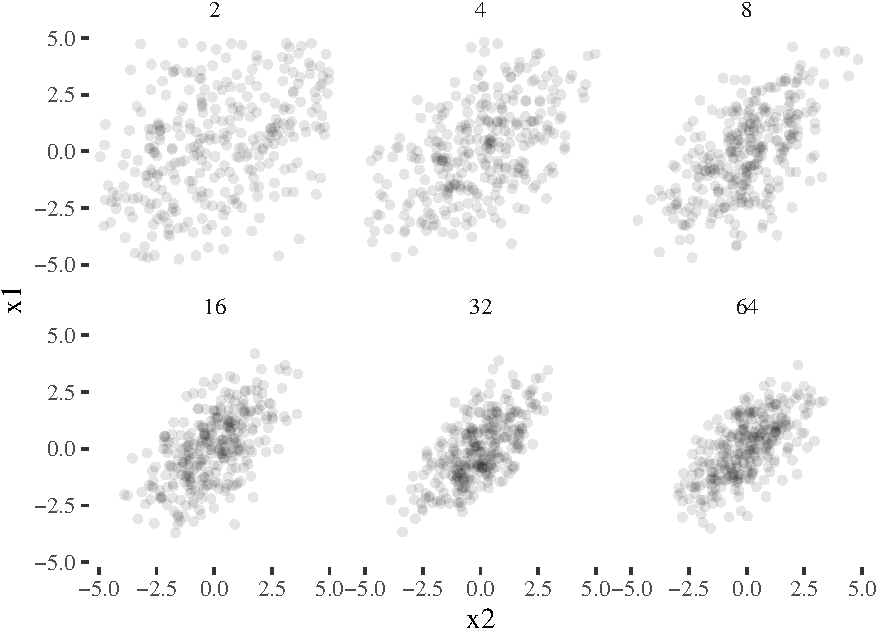
\includegraphics[width=350px]{figure-latex/scatter-1.pdf}
\caption[Scatterplot of simulated practices]{\label{scatter} The figure shows a scatterplot of the distribution of $300$ observations of $x_1$ and $x_2$ for different levels of optimality, $O = 2, 4, 8, 16, 32, 64$. The complementarity effect is present ($\beta_{12} = 0.25$). The decreasing marginal costs are set as $\delta_1 = \delta_2 = 1$. The effect of the environmental variable only affects one of the choices
($\gamma_1 = .33, \gamma_2 = 0$). The unobserved variation parameters are set at $\sigma_{\epsilon_1} = \sigma_{\epsilon_2} = \sigma_{\nu} = 1.$} 
\end{figure}

\subsection{Calibration to Empirical Studies}\label{calibration-to-empirical-studies}

In order to calibrate the simulation, we collect the correlations of published survey studies that cite \citet{grabner_management_2013} and have an interdependency hypothesis. The median number of observations in the studies is 250 and the average is 265. To give the methods the benefit of the doubt, the simulation will create samples of 300 firm observations where each observation follows the algorithm above. Next, we collect the correlation matrix from 9 studies that report full correlation matrices with correlations between practices, and between practices and environmental factors \citep{dekker_collaborative_2016, grabner_incentive_2014, grabner_cost_2016, bedford_configurations_2015, heinicke_examination_2016, bedford_performance_2019, abernethy_are_2015, sponem_exploring_2016, samagaio_management_2018}. To get an estimate of observed correlations in empirical studies, we calculate the median and 90th percentile absolute correlation between practices and between a practice and a contingency factor. We consider the median value of those statistics to be typical for studies on interdependencies in management accounting. The median absolute correlation between two practices is $0.22$ and the median 90th percentile correlation is $0.39$. The median absolute correlation between a practice and an environmental factor is $0.16$ and the median 90th percentile correlation is $0.30$

To illustrate the effect of the optimality parameter and the strength of the associations generated by the simulation algorithm, we generate 100 samples with each 300 observations under the baseline scenario outlined above for 6 levels of optimality: $O \in  \{2, 4, 8, 16, 32, 64\}$. For each sample, we calculate three statistics to illustrate that the simulated samples reflect a typical management accounting study. We plot the statistics for each simulated sample in Figure \ref{calibration}. The first statistic is the correlation between $x_1$ and $x_2$ (Panel A) and the second is the correlation between $x_1$ and $z$ (Panel B). The absolute correlation between $x_1$ and $x_2$ varies between 0 and .5 and is smaller than the median 90th percentile ($.39$) in a typical study except at the higher levels of optimality. Similarly the correlation between $x_1$ and $z$ varies between 0 and .4 and is smaller than the median 90th percentile (.30) in a typical study except at the higher levels of optimality. Hence, we conclude that the associations in our simulations are representative for the management accounting literature. 

The third statistic is the non-optimality ratio and quantifies the extent to which deviations from the optimal level $x^*_1|z$ cannot be explained by the optimality conditions \eqref{eq:optimal}.\footnote{The total deviations from the optimal level conditional on the contingency factor is calculated as the sum of $(x_1 - E(x_1^*|z))^2$ for each observation in the sample, where $E(x_1^*|z)$ is given by the optimality condition \eqref{eq:optimal}. The amount of variation explained by the unobserved factors, $\epsilon_1$ and $\epsilon_2$, can also be calculated from the optimality conditions \eqref{eq:optimal}, i.e., $Var(x_1^*|z) = \frac{\delta_2^2 \sigma_{\epsilon_1}^2 + \beta_{12}^2 \sigma_{\epsilon_1}^2}{(\delta_1 \delta_2 - \beta_{12}^2)^2}$
The non-optimality ratio is then calculated as the ratio between the deviations from optimality not explained by the unobserved factors and the total deviations from optimality.} The non-optimality ratio measures how much of the variation in the practices is caused by the algorithmic search process and how far the practices in a sample are from the optimal levels. The resulting ratio is comparable to an $R^2$ statistic because the non-optimality ratio equals $1$ when the difference between $x_1$ and $x^*_1$ can be fully explained by the absence of optimality in a sample, and the ratio equals $0$ when $x_1 = x^*_1$. Figure \ref{calibration} Panel C shows the ratio for the 100 samples for different levels of the optimality parameter $O$. The ratio declines for higher values of the optimality parameter and for all values of $O$ at least $20\%$ of the variation cannot be explained by the optimality condition. In other words, the generated samples always have substantial deviations from optimal practices, which should give performance specifications a chance of detecting performance differences between optimal and sub-optimal accounting systems. 

\begin{figure}
\centerfloat
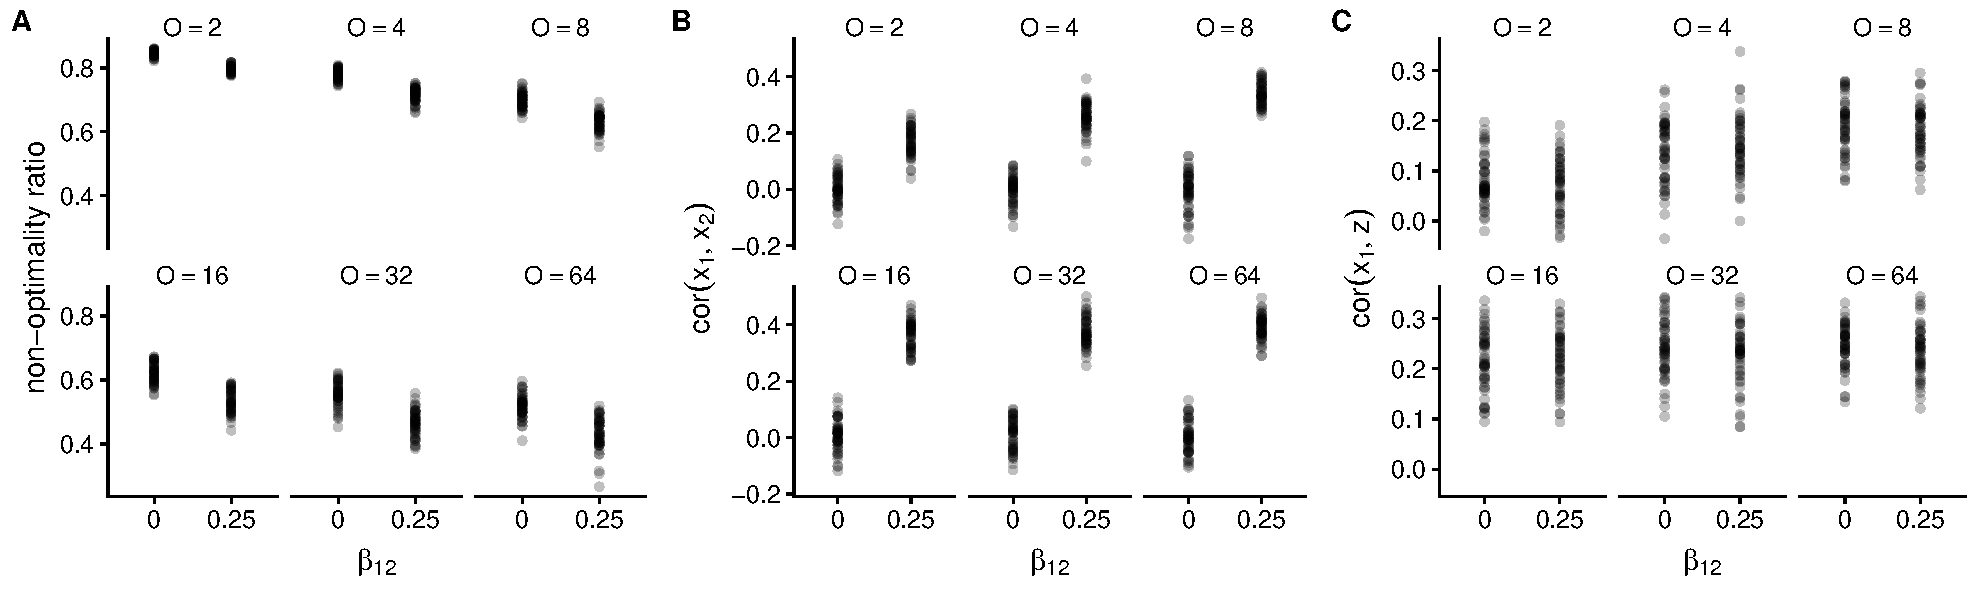
\includegraphics[width=450px]{figure-latex/sample_descriptives.pdf}
\caption[Calibration of Simulated Samples]{\label{calibration} The figure shows the value of the correlation between $\mathbf{x_1}$ and $\mathbf{x_2}$ (Panel A), the correlation between $\mathbf{x_1}$ and $\mathbf{z}$ (Panel B), and the non-optimality ratio (Panel C),  for 100 samples for 6 different levels (2, 4, 8, 16, 32, 64) of the optimality parameter, $O$. The complementarity effect is either present ($\beta_{12} = 0.25$) or absent ($\beta_{12} = 0$). The decreasing marginal costs are set as $\delta_1 = \delta_2 = 1$. The effect of the environmental variable only affects one of the choices
($\gamma_1 = .33, \gamma_2 = 0$). The unobserved variation parameters are set at $\sigma_{\epsilon_1} = \sigma_{\epsilon_2} = \sigma_{\nu} = 1.$}
\end{figure}

\subsection{Power and Type I Error}
In the next section, we will compare the power and Type I error rate of the four specifications when varying the optimality parameter, $O$. Because the accounting literature is concerned with testing the hypothesis that there is a (no) complementarity between two management control practices, a focus on power and error rates is appropriate. For completeness, we repeat the four specifications here
\begin{align*} 
x_1 &= \beta_1^d + \beta_{12}^d x_2 
        + \gamma_{1}^d z
        + \epsilon^d \\
y &=  \beta^{p1}_0 + (\beta^{p1}_{1} + \gamma_1^{p1} z )x_1 
						+ (\beta_{2}^{p1} + \gamma_2 z ) x_2 
                        + \beta_{12}^{p1} x_1 x_2 
                        + \delta_1^{p1} x^2_1 + \delta_2^{p1} x^2_2 
                        + \alpha^{p1} z
                        + \nu^{p1} \\
 y &=  \beta^{p2}_0 + (\beta^{p2}_{1} + \gamma_1^{p2} z )x_1 
						+ (\beta_{2}^{p2} + \gamma_2 z ) x_2 
                        + \beta_{12}^{p2} x_1 x_2 
                        + \alpha^{p2} z
                        + \nu^{p2} \\
 y &=  \beta^{p3}_0 + \beta^{p3}_{1} x_1 
						+ \beta_{2}^{p3} x_2 
                        + \beta_{12}^{p3} x_1 x_2 
                        + \alpha^{p3} z
                        + \nu^{p3}
\end{align*}
The $\beta_{12}$ coefficients for each specification provide the test for the presence of an interdependency. The simulation generates 1000 samples for each combination of parameters. For each combination, we report the distribution of the t-statistic for the interdependency coefficient and compare it to the traditional cut-off value for the $5\%$ level of significance ($|t| > 1.97$). We also calculate the power and Type I error rate of the specifications to investigate the performance of the four specifications in more detail. The power is the percentage of samples with a complementarity effect where the p-value is lower than $0.05$ and the estimated coefficient is positive.\footnote{An important caveat is that the power of a study will also be influenced by the size of the effect, measurement error, random variation, and the number of observations in the study. In the simulations, we assumed a fixed effect ($\beta_{12} = 0.25$), no measurement error, fixed the parameters that control random variation, $\sigma_{\epsilon_1}$, $\sigma_{\epsilon_2}$, and $\sigma_{\nu}$, and the number of observations per sample. As a result, the absolute percentages in the results should be interpreted with caution. This study is mainly interested in the relative differences between specifications, focusing on a clean setting and a fair comparison.} The Type I error is the percentage of samples without a complementarity effect where the p-value is lower than $0.05$ (irrespective of the sign of the estimated coefficient). 

\section{Results}
\subsection{Performance and Demand Specification}\label{performance-and-demand-function-approach}


\subsubsection{Power}\label{Power}
Figure \ref{main} Panel A shows a boxplot for the distribution of t-statistics for each type of test and each combination of parameters. The dot of the boxplot shows the median t-statistic of the 1000 samples, the gap between the whiskers shows the interquartile range, and the ends of the whiskers show the minimum and maximum t-statistic. Each boxplot can be compared to the zero line and the dotted lines representing a $95\%$ confidence interval around a null effect. When $\beta_{12} = 0.25$, we expect the distribution of the t-statistic to be above the dotted lines because it shows that the test reliably reports a significant positive interdependency (power).  

Figure \ref{main} Panel A reveals the basic trade-off between the demand specification and the performance specification: with low levels of optimality the performance function is more likely to detect a true complementarity effect while the demand function is more likely to detect a true complementarity effect with high levels of optimality \citep{grabner_management_2013, aral_three-way_2012, johansson_testing_2018}. The boxplots of the t-statistics are above the $95\%$ confidence interval for the \emph{performance 1} specification with lower levels of optimality and they are above the $95\%$ confidence interval for the \emph{demand} specification for higher levels of optimality.

Interestingly, even at relatively low levels of optimality, i.e., $O = 4$, the \emph{demand} specification has similar power to the \emph{performance 1} specification. Figure \ref{calibration} shows that with $O=4$ the optimality condition can at best explain $40\%$ of the variation in the distance between the observed level of the practices and the optimal level of the practices. This implies that, as long as firms avoid the worst possible combinations of management accounting practices, the demand specification is more likely to detect a true effect.

The \emph{performance 2} specification without the quadratic terms fares worse than the \emph{performance 1} specification at lower optimality levels. The boxplots fall almost entirely within the $95\%$ confidence interval around $0$ with low levels of optimality and a true effect. The omission of the quadratic terms decreases the ability of the \emph{performance 2} specification to detect a real interdependency ($\beta_{12} = 0.25$) at lower levels of optimality. Surprisingly, the \emph{performance 2} specification has more power to detect a real interdependency than the \emph{performance 1} specification at higher levels of optimality. The counterintuitive reason for this is that the bias associated with the omission of the quadratic terms (see equation \ref{eq:omitted}) inflates the estimate of the complementarity with a factor proportional to the correlation between $x_1$ and $x_2$. In effect, the bias in \emph{performance 2} inadvertently picks up the same signal, i.e. the relation between the two practices, as the demand specification. Nevertheless, in terms of power, the \emph{demand} specification dominates the \emph{performance 2} specification. The \emph{performance 3} specification performs as poorly as the \emph{performance 2}  specification, in terms of power. 

\begin{figure}
\centerfloat
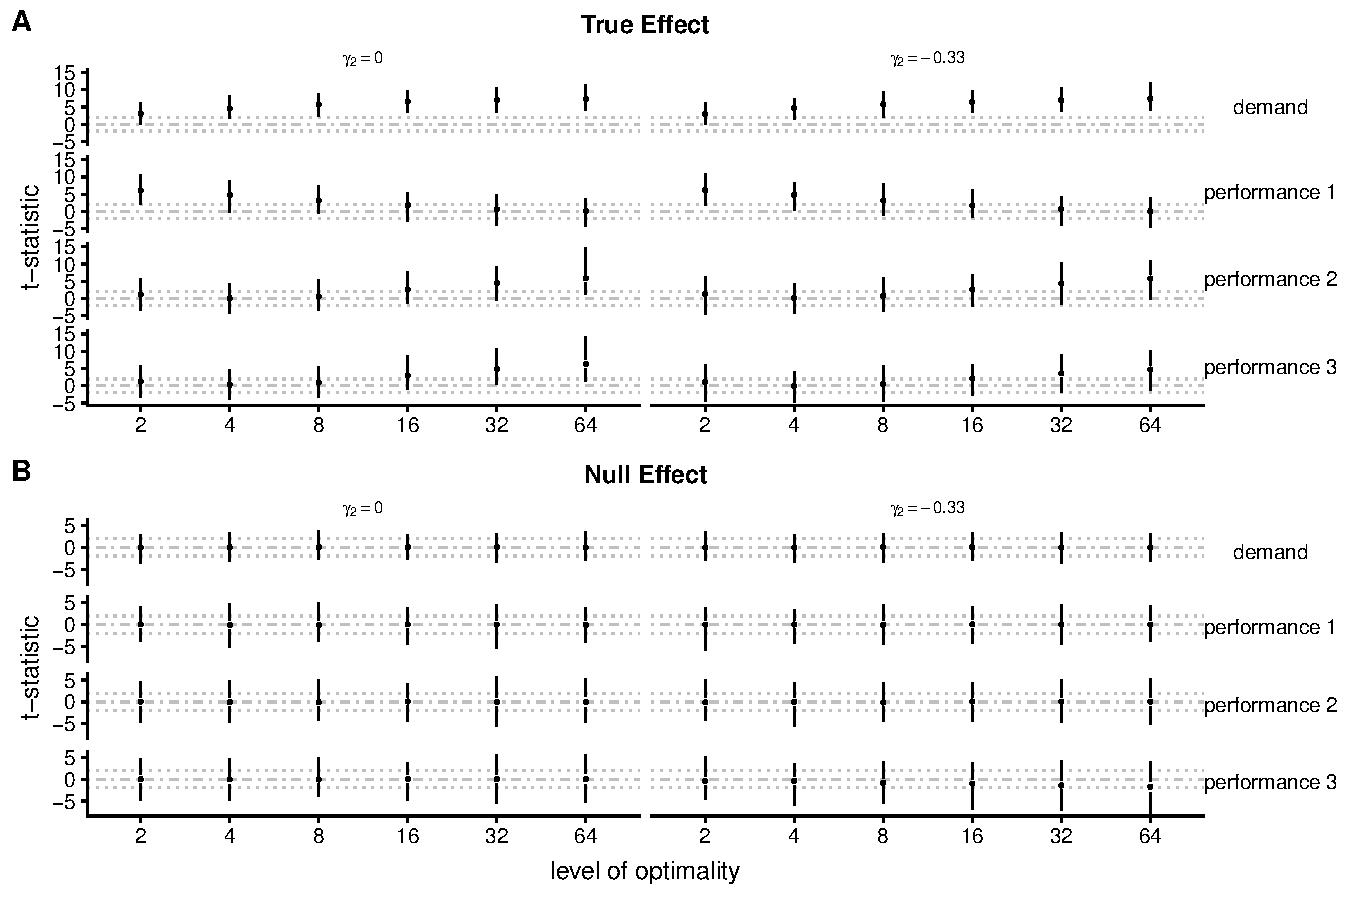
\includegraphics[width=450px]{figure-latex/main_new_plot.pdf}
\caption[Error Rate  and Power of Demand and Performance Specification]
{\label{main} t-statistic of the performance and demand specification to test
for complementarities when there is a complementarity effect ($\beta_{12} = .25$)
in Panel A or a null effect ($\beta_{12} = 0$) in Panel B. The boxplots represent the median (the dot), the interquartile range (the gap), and the minimum and maximum (the whiskers). $O$ is varied between 2, 4, 8, 16, 32, and 64. The effect of the environmental variable, $\mathbf{z}$, on the second choice is either absent ($\gamma_1 = .33,   \gamma_2 = 0$), or negative ($\gamma_1 = .33$ and $\gamma_2 = -.33$).}
\end{figure}

\begin{table}[ht]
\centering
\begingroup\footnotesize
\begin{tabular}{lrlrrrrrr}
  \hline
specification & $\gamma_2$ & statistic & 2 & 4 & 8 & 16 & 32 & 64 \\ 
  \hline
demand & -0.33 & type I & 0.05 & 0.05 & 0.05 & 0.04 & 0.04 & 0.05 \\ 
  demand & 0.00 & type I & 0.05 & 0.04 & 0.05 & 0.04 & 0.04 & 0.04 \\ 
  demand & 0.33 & type I & 0.04 & 0.04 & 0.05 & 0.04 & 0.05 & 0.04 \\ 
  performance~1 & -0.33 & type I & 0.17 & 0.14 & 0.18 & 0.16 & 0.15 & 0.14 \\ 
  performance~1 & 0.00 & type I & 0.16 & 0.17 & 0.17 & 0.15 & 0.13 & 0.15 \\ 
  performance~1 & 0.33 & type I & 0.16 & 0.15 & 0.15 & 0.15 & 0.15 & 0.12 \\ 
  performance~2 & -0.33 & type I & 0.20 & 0.19 & 0.18 & 0.16 & 0.21 & 0.22 \\ 
  performance~2 & 0.00 & type I & 0.21 & 0.20 & 0.18 & 0.15 & 0.18 & 0.22 \\ 
  performance~2 & 0.33 & type I & 0.19 & 0.19 & 0.17 & 0.16 & 0.20 & 0.22 \\ 
  performance~3 & -0.33 & type I & 0.21 & 0.20 & 0.22 & 0.30 & 0.40 & 0.48 \\ 
  performance~3 & 0.00 & type I & 0.20 & 0.20 & 0.18 & 0.16 & 0.19 & 0.25 \\ 
  performance~3 & 0.33 & type I & 0.20 & 0.19 & 0.21 & 0.28 & 0.39 & 0.47 \\ 
  demand & -0.33 & power & 0.84 & 1.00 & 1.00 & 1.00 & 1.00 & 1.00 \\ 
  demand & 0.00 & power & 0.84 & 1.00 & 1.00 & 1.00 & 1.00 & 1.00 \\ 
  demand & 0.33 & power & 0.81 & 1.00 & 1.00 & 1.00 & 1.00 & 1.00 \\ 
  performance~1 & -0.33 & power & 1.00 & 0.98 & 0.82 & 0.43 & 0.16 & 0.06 \\ 
  performance~1 & 0.00 & power & 1.00 & 0.98 & 0.82 & 0.43 & 0.19 & 0.07 \\ 
  performance~1 & 0.33 & power & 1.00 & 0.98 & 0.82 & 0.41 & 0.15 & 0.07 \\ 
  performance~2 & -0.33 & power & 0.37 & 0.10 & 0.20 & 0.70 & 0.95 & 0.99 \\ 
  performance~2 & 0.00 & power & 0.32 & 0.10 & 0.22 & 0.69 & 0.96 & 0.99 \\ 
  performance~2 & 0.33 & power & 0.36 & 0.09 & 0.21 & 0.67 & 0.96 & 0.99 \\ 
  performance~3 & -0.33 & power & 0.31 & 0.07 & 0.14 & 0.55 & 0.85 & 0.94 \\ 
  performance~3 & 0.00 & power & 0.34 & 0.12 & 0.27 & 0.76 & 0.97 & 0.99 \\ 
  performance~3 & 0.33 & power & 0.45 & 0.20 & 0.50 & 0.92 & 1.00 & 1.00 \\ 
   \hline
\end{tabular}
\endgroup
\caption{Type I error rates and power for the demand and
             performance function approaches at different levels optimality: 
             2, 4, 8, 16, 32, 64. The parameters are the same as in Figure 
             \ref{basic}.} 
\label{basic-error}
\end{table}


To evaluate the demand and performance specifications in more detail, we report the power of the four specifications in Table \ref{tab:main-table}. The results show that the "optimality trade-off" between the demand specification and the performance specification that is discussed in the literature \citep{grabner_management_2013, aral_three-way_2012, johansson_testing_2018} is really a second order problem. Both the \emph{demand} and the \emph{performance 1} specification are able to detect a true interdependency with more than $80\%$ probability for low to medium levels of optimality. However, the \emph{demand} specification is more likely to detect a true effect at higher levels of optimality. Strictly speaking, the \emph{demand} specification is more likely to detect a true effect at all levels of optimality but the lowest level, i.e., at \(O = 2\). From a power perspective, the \emph{demand} specification dominates the \emph{performance 1} specification. Finally, the \emph{performance 2} and \emph{performance 3} specifications are not able to detect the true interdependency for most of the parameter space under investigation, except at high levels of optimality. As stated before, the power that these specifications have at higher levels of optimality is due to the bias from omitting the quadratic terms which depends on the correlation between $x_1$ and $x_2$. While this bias helps with increasing power, it comes at the cost of high Type I error rates, as we show next.

\subsubsection{Type I error}\label{Type I error}
Figure \ref{main} Panel B shows a boxplot for the distribution of t-statistics for each type of test and each combination of parameters. When $\beta_{12} = 0$, we expect the distribution of the t-statistic to be centred on $0$, as well as $95\%$ of the distribution to be between the two dotted lines. When the distribution is not centred on $0$, the test is biased. When the distribution is too wide, the test reports too many significant interdependencies in the absence of a true effect (Type I error).

Figure \ref{main} Panel B shows that the demand specification, the theoretically appropriate \emph{performance 1} and the \emph{performance 2} specifications have an average t-statistic close to $0$ in the absence of an interdependency. The boxplots are centred around the zero line for these three specifications. Recall that the omission of the quadratic terms does not bias the estimate of a complementarity in the absence of the complementarity ($\beta_{12} = 0$).

The \emph{performance 3} specification fares worse than all other specifications. The omission of the interaction terms \(x_1z\) and \(x_2z\) biases the estimate of the interdependency when $\gamma_1 \gamma_2 \neq 0$. The bias can be easily seen in Figure \ref{main} Panel B. The distribution of t-statistics for samples without a complementarity effect no longer centres on $0$ when the environmental factor has a contingency effect on the performance of both practices and the bias increases with higher levels of optimality. The bias is negative when $\gamma_2$ is negative and positive when $\gamma_2$ is positive. The latter case is not depicted in Figure \ref{main}.

To evaluate the Type I errors of the demand and performance specifications in more detail, we report the percentage of samples for which the estimate of $\beta_{12}$ is significantly positive or negative  in Table \ref{tab:main-table}. Under the parameters in the simulation study, the \emph{demand} specification has Type I error rates slightly below or equal to $0.05$. This means that the number of false positives are consistent with the nominal p-value of $5\%$. The theoretically appropriate \emph{performance 1} specification tends to have error rates elevated by a factor two to three relative to the \emph{demand} specification. The most worrying results are for the \emph{performance 2} and \emph{3} specifications. Dropping the quadratic effects increases the error rates in the \emph{performance 2} specification to around $.20$, four times the nominal error rate. The most commonly used specification in the literature, \emph{performance 3}, has even higher Type I error rates that increase with higher levels of optimality and when the environmental factor has a contingency effect on both practices. The misspecification in \emph{performance 3} leads to a bias in the estimated coefficient for the interdependency and thus the t-statistic. In conclusion, given the parameters in the simulation study only the \emph{demand} specification rejects the null hypothesis at nominal $5\%$ level of significance. The theoretically derived \emph{performance 1} specification has elevated error rates, and the two other performance specifications are even more vulnerable to false positives.

\subsubsection{Take-away of baseline simulation}\label{Take-away of baseline simulation}
The results of the simulation using the baseline model reveal the following: In contrast to arguments put forward in the literature, the \emph{demand} specification has significant power at all levels of optimality. The assumption regarding the level of optimality to decide between specifications is a second-order consideration. Unless the researcher can argue that the sample has quasi-random assignment of practices, the demand specification should be preferred. In addition, the Type I error rates of the \emph{demand} specification are consistent with the nominal p-value of $5\%$. The theoretically appropriate \emph{performance 1} specification has significant power at low to medium levels of optimality, which is in line with arguments in the literature. However, the problem with this specification is the elevated Type I errors. These Type I errors only get worse once the performance specification is misspecified, as in \emph{performance 2} and \emph{performance 3}.

One way to interpret the elevated Type I errors of the performance specifications is to think about how a reader should react when observing a study with a significant positive interaction \(x_1 x_2\). To demonstrate the problems with the \emph{performance 3} specification, we provide one dramatic example for \(O = 4\) and \(\gamma_2 = -0.33\). If we assume that a priori, we are indifferent between a null effect and a true interdependency of \(\beta_{12} = 0.25\), and we observe one study that reports a significant positive interaction \(x_{1} x_{2}\), the study is more likely to be from a sample where the null holds than from a sample where there is a true interdependency!

In sum, the results regarding power and Type I errors indicate that the \emph{demand} specification performs better on both dimensions compared to all three performance specifications.

\subsection{Parameter Variations}\label{parameter-variations}

In this section, we explore the robustness of the above conclusions to variations in the parameters of the objective functions. Given the large number of possible variations, we restrict ourselves to theoretically driven comparisons. We do not consider the condition $O = 64$ in the following results because generating a sample of $O = 64$ is as computationally costly as generating a sample of each of the other levels of optimality. Furthermore, the results in Table \ref{tab:main-table} and Figure \ref{main} show that the results do not qualitatively differ between $O = 32$ and $O = 64$.

\subsubsection{Performance Variation}\label{performance-variation}

We first investigate whether an increase in the variance of performance, $\sigma_{\nu}$, changes the above conclusions. This increase in variance has two possible effects. The first effect is a decrease in the importance of the management practices for performance, which decreases the power of the performance specification. The second effect follows from the first. When the management practices are less important, the level of optimality effects are less pronounced, and the correlations between $x_1$, $x_2$, and $z$ are weaker, which in turn decreases the power of the demand specification and the omitted correlated variable bias in the \emph{performance 2} and \emph{performance 3} specification.

To investigate the role of $\sigma_{\nu}$, we vary the parameter between 1, 2, and 4 while keeping the other parameters the same as in Figure \ref{main}. For clarity of exposition, we limit the number of optimality variations ($O = 2, 8, 32$) and the number of variations of the contingency effect $x_2 z$ ($\gamma_2 = -.33$) in Figure \ref{noise}.

\begin{figure}
\centerfloat
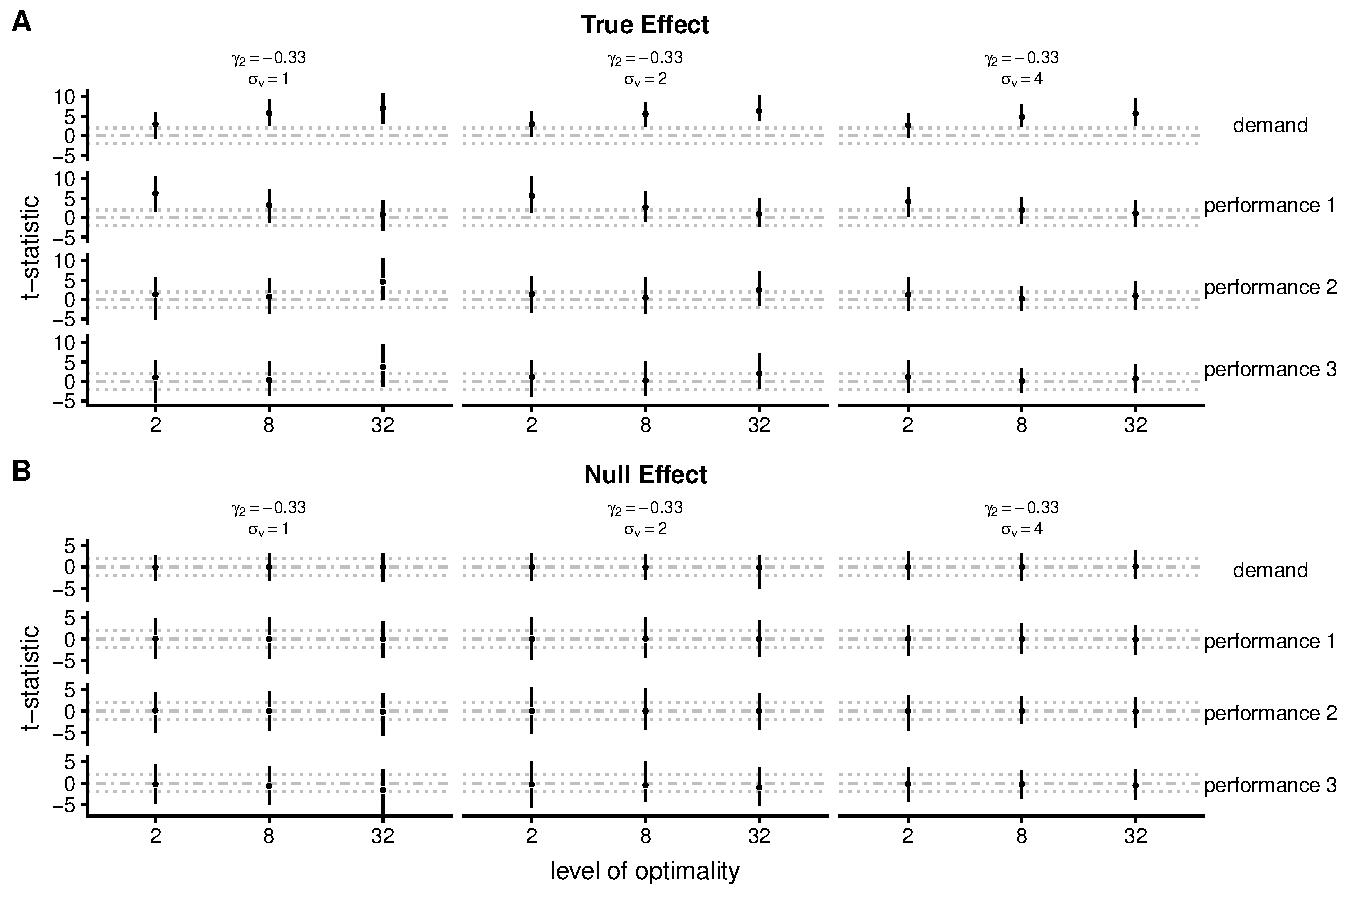
\includegraphics[width=450px]{figure-latex/noise_new_plot.pdf}
\caption[Error Rate and Power with Increasing Levels of Variability in Performance]
{\label{noise} t-statistic of the performance and demand specification to test
for complementarities when there is a complementarity effect ($\beta_{12} = .25$)
in Panel A or a null effect ($\beta_{12} = 0$) in Panel B. The boxplots represent the median (the dot), the interquartile range (the gap), and the minimum and maximum (the whiskers). $O$ is varied between 2, 8, 32. The effect of the environmental variable, $\mathbf{z}$, on the second choice is negative ($\gamma_1 = .0.33$ and $\gamma_2 = -.33$).}
\end{figure}

\begin{table}[ht]
\centering
\begingroup\footnotesize
\begin{tabular}{lrlrrr}
  \hline
specification & $\gamma_2$ & statistic & 2 & 8 & 32 \\ 
  \hline
demand & -0.33 & type I & 0.04 & 0.05 & 0.04 \\ 
  demand & 0.33 & type I & 0.05 & 0.05 & 0.05 \\ 
  performance~1 & -0.33 & type I & 0.09 & 0.06 & 0.06 \\ 
  performance~1 & 0.33 & type I & 0.08 & 0.06 & 0.07 \\ 
  performance~2 & -0.33 & type I & 0.12 & 0.07 & 0.07 \\ 
  performance~2 & 0.33 & type I & 0.13 & 0.07 & 0.07 \\ 
  performance~3 & -0.33 & type I & 0.12 & 0.09 & 0.10 \\ 
  performance~3 & 0.33 & type I & 0.14 & 0.08 & 0.11 \\ 
  demand & -0.33 & power & 0.75 & 1.00 & 1.00 \\ 
  demand & 0.33 & power & 0.75 & 1.00 & 1.00 \\ 
  performance~1 & -0.33 & power & 0.98 & 0.53 & 0.20 \\ 
  performance~1 & 0.33 & power & 0.97 & 0.49 & 0.17 \\ 
  performance~2 & -0.33 & power & 0.30 & 0.06 & 0.16 \\ 
  performance~2 & 0.33 & power & 0.32 & 0.05 & 0.14 \\ 
  performance~3 & -0.33 & power & 0.25 & 0.04 & 0.12 \\ 
  performance~3 & 0.33 & power & 0.39 & 0.11 & 0.37 \\ 
   \hline
\end{tabular}
\endgroup
\caption{Type I error rates and power for the demand and
             performance specifications at different levels optimality: 
             2, 8, 32. The parameters are the same as in Figure \ref{noise}.
             Only the results for $\sigma{nu} = 4$ are reported} 
\label{noise-table}
\end{table}


The results in Figure \ref{noise} and Table \ref{tab:noise-table} are qualitatively the same as the results in Figure \ref{main} and Table \ref{tab:main-table}. Surprisingly, in the presence of an interdependency, the increase in performance variance hardly affects the power of the \emph{demand} specification. At all but the lowest level of optimality, the \emph{demand} specification correctly identifies the interdependency for every simulated sample with a real interdependency, although the t-statistics decrease with higher performance variance. The drop-off in the t-statistic is steeper for the \emph{performance 1} specification to the extent that power drops to around \(20\%\) when \(O = 32\) and \(\sigma_{\nu} = 4\). In summary, these results indicate that the impact of increasing the performance variance is a major decrease in the power of the performance specifications and only a minor decrease in the power of the demand specification.

Regarding Type I errors, we find that the \emph{demand}, the \emph{performance 1}, and the \emph{performance 2} specification are unbiased. In addition, the \emph{demand} specification has false positive rates below or close to the nominal rates, while the \emph{performance 1} specification still has elevated Type I error rates. The \emph{performance 2} and \emph{performance 3} specification exhibit the same problem as before, namely elevated false positive rates as a result of misspecification. The increase in unobserved performance variation does lessen the impact of this bias. In summary, the conclusion that the demand specification outperforms the performance specifications is not changed when the noise in performance increases.

\subsubsection{Marginal Costs}\label{marginal-cost}
 
In this section, we vary the size of the increase in marginal costs, $\delta_1 = \delta_2$. We keep the parameters equal for both management control practices but they become smaller in size. There are two consequences of lowering the increase in marginal costs. First, decreasing $\delta_1 = \delta_2$ increases the importance of the complementarity between the management control practices. Second, the bias from omitting the quadratic terms is smaller. In the baseline scenario, we used $\delta_1 = \delta_2 = 1$. In this section, we compare the baseline scenario to two other values, i.e., $0.25$ and $0$. $\delta_1 = \delta_2 = .25$ is the largest value for which the parameters violate the second-order optimality condition $\beta_{12} < \sqrt{\delta_1 \delta_2}$. When the second-order optimality condition is violated, the optimal level for the practices will cluster towards 5 and -5 and away from  0. The extreme case is when $\delta_1 = \delta_2 = 0$ which may impede the inference by the \emph{demand} specification even further. 

Figure \ref{delta} and Table \ref{tab:delta-table} report the power and Type I error rate of the different specifications for samples of firms with slowly increasing ($\delta_i = .25$) or fixed marginal costs ($\delta_i = 0$). Because the results showed no trends for different values of $\gamma_2$, we aggregated the results over all values of $\gamma_2$ in the table. The power of the \emph{demand} specification is generally better for all but the lowest level of optimality, while the \emph{performance 1} specification suffers from steep decreases in power with higher levels of optimality. The \emph{demand} specification does suffer from slightly elevated false positives when the marginal costs of the choices are constant or only increasing slowly. However, the overall conclusions are unaffected.

\begin{figure}
\centerfloat
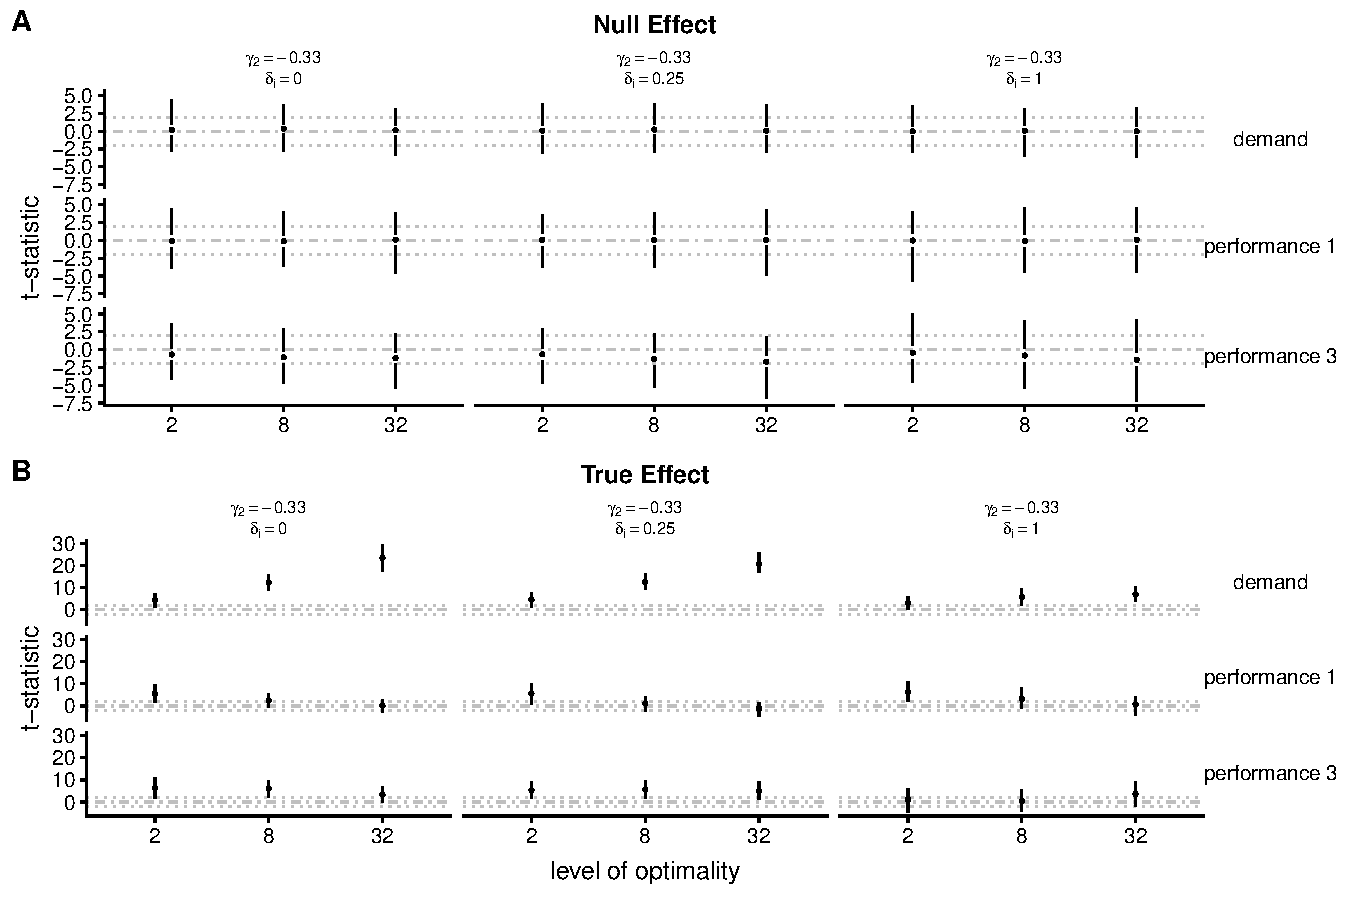
\includegraphics[width=450px]{figure-latex/delta_new_plot.pdf}
\caption[The Error Rate and Power with Different Levels of Marginal Costs]
{\label{delta} t-statistic of the performance and demand specification to test
for complementarities when there is a complementarity effect ($\beta_{12} = .5$)
in Panel A or a null effect ($\beta_{12} = 0$) in Panel B. The boxplots represent the median (the dot), the interquartile range (the gap), and the minimum and maximum (the whiskers). $N$ is varied between 2, 8, 32. The effect of the environmental variable, $\mathbf{z}$, on the second choice is negative ($\gamma_1 = .33$ and $\gamma_2 = -.33$). The change in marginal costs varied between $\delta_1 = \delta_2 = 0, .25, 1$}
\end{figure}

\begin{table}[ht]
\centering
\begingroup\footnotesize
\begin{tabular}{lrrlrrr}
  \hline
specification & $\gamma_2$ & $\delta_i$ & statistic & 2 & 8 & 32 \\ 
  \hline
demand & 0.33 & 0.00 & type I & 0.06 & 0.06 & 0.04 \\ 
  demand & 0.33 & 0.25 & type I & 0.06 & 0.05 & 0.05 \\ 
  demand & 0.33 & 1.00 & type I & 0.04 & 0.05 & 0.05 \\ 
  performance~1 & 0.33 & 0.00 & type I & 0.11 & 0.08 & 0.07 \\ 
  performance~1 & 0.33 & 0.25 & type I & 0.13 & 0.09 & 0.11 \\ 
  performance~1 & 0.33 & 1.00 & type I & 0.14 & 0.16 & 0.13 \\ 
  demand & 0.33 & 0.00 & power & 0.99 & 1.00 & 1.00 \\ 
  demand & 0.33 & 0.25 & power & 1.00 & 1.00 & 1.00 \\ 
  demand & 0.33 & 1.00 & power & 0.84 & 1.00 & 1.00 \\ 
  performance~1 & 0.33 & 0.00 & power & 1.00 & 0.74 & 0.01 \\ 
  performance~1 & 0.33 & 0.25 & power & 1.00 & 0.24 & 0.00 \\ 
  performance~1 & 0.33 & 1.00 & power & 1.00 & 0.83 & 0.16 \\ 
   \hline
\end{tabular}
\endgroup
\caption{Type I error rates and power for the \emph{demand} and
             \emph{performance 1} specification at different levels optimality: 
             2, 8, 32. The parameters are the same as in Figure \ref{delta}.
             Only the results for $\gamma_{2} = 0.33$ are reported} 
\label{delta-table}
\end{table}


\subsubsection{Binary Practices}\label{binary-practices}

An alternative approach to deal with accounting practices with fixed or decreasing marginal costs is to treat them as binary decisions, because the optimal decision will either be to use the practice to its full extent or not use it at all. When the accounting practices are binary, the quadratic terms in the \emph{performance 1} specification are no longer identified. Hence, we will compare the \emph{demand} with the \emph{performance 2} specification. In the \emph{demand} specification, we have to take into account that the dependent variable is now a binary outcome. Hence, we compare the linear probability model we have used so far, to the logit and probit estimates of the same specification. However, these alternative estimation methods should produce the same results in our setting. 

We simulate new samples for the parameters in the main analysis with the following levels of optimality: 2, 4, 8, 16. The most important change in algorithm \eqref{eq:firm-simulation} is that we generate the accounting choices, $x_i^o$, no longer from a uniform distribution but let them be $-1$ or $1$ with equal probability. We also set the parameters $\delta_1$ and $\delta_2$ equal to $0$.

The results are shown in Table \ref{tab:discrete-table}. Because the results again showed no differential trends for different values of $\gamma_2$, we aggregated the results over all values of $\gamma_2$. The power of the tests is lower for all tests compared to the same parameters in Table \ref{tab:main-table} for continuous accounting practices. As before, we find that at all but the lowest level of optimality, the \emph{demand} specification has more power to detect a true effect, independent of the functional form used to estimate the complementarity. All specifications have similar and acceptable Type I error rates. In this specific case, the \emph{performance 2} specification does not suffer from elevated Type I error rates. As before, with binary practices, we reach the same conclusion that the demand specification is superior to the performance specification as long as firms largely avoid accounting systems where the relation between the practices is the opposite of the optimal relation.

\begin{table}[ht]
\centering
\begingroup\footnotesize
\begin{tabular}{llrrrr}
  \hline
specification & statistic & 2 & 4 & 8 & 16 \\ 
  \hline
demand & type I & 0.06 & 0.06 & 0.05 & 0.05 \\ 
  logit & type I & 0.06 & 0.06 & 0.05 & 0.05 \\ 
  performance~2 & type I & 0.06 & 0.05 & 0.05 & 0.05 \\ 
  probit & type I & 0.06 & 0.06 & 0.05 & 0.05 \\ 
  demand & power & 0.27 & 0.72 & 0.96 & 1.00 \\ 
  logit & power & 0.27 & 0.72 & 0.96 & 1.00 \\ 
  performance~2 & power & 0.52 & 0.44 & 0.23 & 0.09 \\ 
  probit & power & 0.28 & 0.72 & 0.96 & 0.99 \\ 
   \hline
\end{tabular}
\endgroup
\caption{Type I error rates and power for the demand and 
  performance specifications at different levels optimality: 2, 
  4, 8, 16. The results are aggregated over the parameter values 
  of $\gamma_2$ (-0.33, 0, 0.33).} 
\label{discrete-table}
\end{table}


\subsection{Correlated Omitted Variable}\label{correlated-omitted}

In this section, we investigate to what extent an omitted correlated environmental variable affects our conclusions for the \emph{demand} and \emph{performance 1} specification. The baseline simulation showed that the omission of a contingency factor that affects the performance of both practices, as in \emph{performance 3}, leads to Type I errors. However, this correlated omitted variable problem was due to a misspecification, not due to not having access to the data about the variable. To test the vulnerability of the \emph{demand} specification and the \emph{performance 1} specification to spurious correlations in a well designed study, we run the following simulation: We introduce a new unobserved (to the researcher) environmental factor \(w\) that impacts the performance effect of \(x_1\) with \(\theta_1\) and the performance effect of \(x_2\) with \(\theta_2\). 

\begin{figure}
\centerfloat
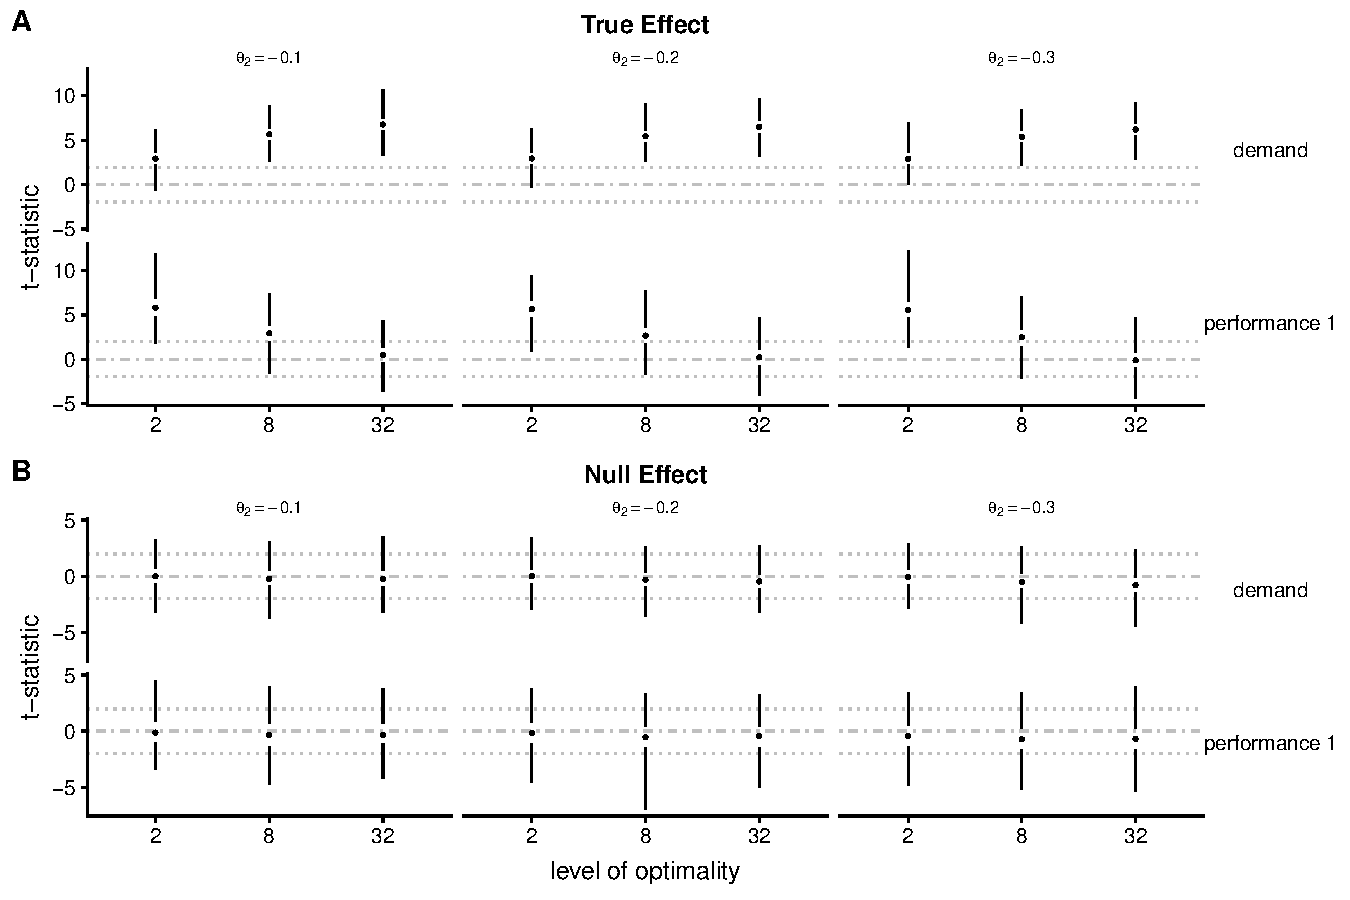
\includegraphics[width=450px]{figure-latex/spurious_new_plot.pdf}
\caption[Error Rate and Power with Unobserved Environmental Variables]
{\label{spurious} t-statistic of the performance and demand specification to test
for complementarities when there is complementarity effect ($\beta_{12} = .25$),
in Panel A or a null effect ($\beta_{12} = 0$) in Panel B. The boxplots represent the median (the dot), the interquartile range (the gap), and the minimum and maximum (the whiskers). $O$ is varied between 2, 8, 32. The effect of the unobserved environmental variable, $\mathbf{w}$, on the choices varies from a strong correlation ($\theta_1 = .3$, $\theta_2 = -.3$), a medium correlation ($\theta_1 = .3$ and $\theta_2 = -.2$), or a weak correlation ($\theta_1 =.3$, $\theta_2 = -.1$).}
\end{figure}

\begin{table}[ht]
\centering
\begingroup\footnotesize
\begin{tabular}{lrlrrr}
  \hline
specification & $\theta_2$ & statistic & 2 & 8 & 32 \\ 
  \hline
demand & -0.30 & power & 0.84 & 1.00 & 1.00 \\ 
  demand & -0.20 & power & 0.84 & 1.00 & 1.00 \\ 
  demand & -0.10 & power & 0.86 & 1.00 & 1.00 \\ 
  performance~1 & -0.30 & power & 0.99 & 0.63 & 0.06 \\ 
  performance~1 & -0.20 & power & 0.99 & 0.70 & 0.10 \\ 
  performance~1 & -0.10 & power & 1.00 & 0.76 & 0.11 \\ 
  demand & -0.30 & type I & 0.06 & 0.07 & 0.12 \\ 
  demand & -0.20 & type I & 0.05 & 0.05 & 0.08 \\ 
  demand & -0.10 & type I & 0.04 & 0.05 & 0.06 \\ 
  performance~1 & -0.30 & type I & 0.18 & 0.21 & 0.21 \\ 
  performance~1 & -0.20 & type I & 0.17 & 0.20 & 0.18 \\ 
  performance~1 & -0.10 & type I & 0.14 & 0.18 & 0.16 \\ 
   \hline
\end{tabular}
\endgroup
\caption{Type I error rates and power for the \emph{demand} and
             \emph{performance 1} specification at different levels of 
             optimality: 2, 8, 32. The parameters are the same as in Figure 
             \ref{spurious}.} 
\label{spurious-table}
\end{table}


We set the parameters assuming a well designed study that controls for most but not all of the environmental factors affecting the performance of both choices. Based on the nine studies in the calibration section, we set values for the contingency effect of the unobserved factor that reflect a large ($\theta_1 = 0.3, \theta_2 = -0.3$), medium ($\theta_1 = 0.3, \theta_2 = -0.2$), and small ($\theta_1 = 0.3, \theta_2 = -0.1$) spurious correlation. The previous methodology literature has long argued that an omitted environmental factor will bias the demand specification. The negative bias due to the omitted correlated variable increases the probability of reporting a substitution effect in the absence of a true effect and decreases the power to reject the null hypothesis when there is a true complementarity.\footnote{A positive bias, i.e., $\theta_1 \theta_2 > 0$, increases the probability of reporting a complementarity effect in the absence of a true effect. The Type I errors that might occur because of this correlated omitted variable problem are, by construction, identical to those for $\theta_1 \theta_2 < 0$. Using $\theta_1 \theta_2 < 0$ in our simulation allows us to capture two problems at once, i.e., potentially elevated Type I errors and reduced power.}  We theoretically argued above that under the same condition, i.e., $\theta_1 \theta_2 \neq 0$, the performance specification will be biased as well. The results of this simulation reveal to what extent both specifications are vulnerable to this bias.

The results are reported in Figure \ref{spurious} and Table \ref{tab:spurious-table}. These results are consistent with our previous findings. The \emph{demand} specification has at all but the lowest levels of optimality more power to detect a true interdependency than the \emph{performance 1} specification. One logical finding is that the \emph{demand} specification becomes vulnerable to the omitted variable bias and thus higher Type I error rates at higher levels of optimality. This effect is most pronounced with the largest spurious correlation (\(\theta_1 = .3\), \(\theta_2 = -.3\)) and \(O = 32\), where we find that in $12\%$ of the simulations with a null effect the \emph{demand} specification reports a significant effect. This finding reinforces that the \emph{demand} specification will only have appropriate Type I error rates as part of a well designed study that controls for environmental factors that affect both choices, especially when firms adopt the optimal management controls. However, consistent with our arguments, the \emph{performance 1} specification exhibits the exact same bias and, as a result, the \emph{demand} specification still has superior Type I error rates compared to the \emph{performance 1} specification.

\subsection{Robustness and Limitations of the Demand Specification} \label{robustness-demand}

In this section we explore under which part of the parameter space the demand specification is less robust than the performance specification. In addition, we investigate whether our main conclusion that the demand specification generally dominates the performance specification, holds for objective functions with three practices and three complementarities, and for a combination of discrete and continuous practices. There are two main conclusions to this section. First, the principal weakness of the demand specification is elevated Type I error rates when it is optimal for more than half of the sample to choose the maximum level for both practices. This occurs when the practices have no increasing marginal costs (or alternatively, no decreasing marginal returns) and when contingency effects are small. Given how extreme such a worst case scenario is, we believe this result only marginally qualifies our main conclusion. In the majority of the management accounting studies we belief that variation in contingency factors and/or decreasing marginal returns will dominate over the direct benefits of the practices. If this is the case, the demand specification has more power to detect a true complementarity at all but the lowest level of optimality while keeping Type I error rates at the nominal $5\%$ level.

The second conclusion of this section is that the demand specification generally deals well with discrete practices or an objective function with more than two practices and complementarities. Thus, our overall conclusion and recommendations generalise to this expanded objective function. Nevertheless, in this setting the demand specification suffers from the same inflated Type I error rate when it is optimal for more than half of the sample to choose the maximum level for any two practices. Because the decision to adopt a binary practice is inherently all or nothing, the issue is more pronounced for a test of complementarity between two discrete practices. Similarly as before, when the benefits of the practices vary enough in the sample due to contingency effects, the demand specification outperforms the performance specification at all but the lowest level of optimality.

The technical reason for the main weakness of the demand specification is that the corner solution of adopting both practices to their full extent violates the second order optimality condition as discussed in \ref{optimal-level-of-practices}. The three subsections that follow explain the technical details of the simulations and explain how we establish quantitatively that the worst case scenario is unlikely to occur in a typical management accounting setting. The first section investigates an expanded set of parameter combinations to show the robustness of the baseline results in \ref{Take-away of baseline simulation}. Under this simulation, corner solutions are possible for all four combinations and they are all equally likely to occur in the sample.\footnote{The four possible corner solutions are: (1) Fully adopt practice 1 and 2, (2) Fully adopt practice 1 and do not adopt practice 2 at all, (3) fully adopt practice 2 and do no adopt practice 1 at all, and (4) do not adopt practice 1 and 2 at all.} The second section changes the first simulation so that one corner solution (i.e. both practices should be adopted to their full extent) is more likely. The third simulation introduces a third practice in the objective function and allows for discrete practices when one corner solution is more likely. 

\subsubsection{Robustness}

In a first simulation, we vary the following parameters. $\beta_{12}$ equals $0$ or $0.25$. $\delta_1 = \delta_2$ equal $0$, $.25$ or $1$. $\gamma_1 = 0.33$ and $\gamma_2$ equals $0$, $-0.33$, or $0.33$. $\sigma_{\epsilon_1} = \sigma_{\epsilon_2}$ varies between $0.5$, $1$, and $2$ and $\sigma_{\nu}$ equals $1$ or $2$. Note that these parameter combinations no longer reflect the calibration to a typical management accounting study in section \ref{calibration-to-empirical-studies}. For computational reasons, we restrict ourselves to comparing the two theoretically derived specifications: the \emph{demand} specification and the \emph{performance 1} specification.

\begin{table}

\caption{\label{tab:big-basis-table}Power and Type I Error Rate without Main Effects}
\centering
\fontsize{8}{10}\selectfont
\begin{tabular}[t]{lrrrrrrrrrrrrr}
\toprule
\multicolumn{4}{c}{ } & \multicolumn{5}{c}{demand specification} & \multicolumn{5}{c}{performance specification} \\
\cmidrule(l{3pt}r{3pt}){5-9} \cmidrule(l{3pt}r{3pt}){10-14}
Type & $\sigma_{\epsilon_i}$ & $\delta_i$ & $\sigma_{\epsilon_i}$ & 2 & 4 & 8 & 16 & 32 & 2 & 4 & 8 & 16 & 32\\
\midrule
power & 0.5 & 0.00 & 1 & 1.00 & 1.00 & 1.00 & 1.00 & 1.00 & 1.00 & 1.00 & 0.99 & 0.64 & 0.14\\
power & 0.5 & 0.00 & 2 & 1.00 & 1.00 & 1.00 & 1.00 & 1.00 & 1.00 & 1.00 & 0.99 & 0.76 & 0.30\\
power & 0.5 & 0.00 & 4 & 0.98 & 1.00 & 1.00 & 1.00 & 1.00 & 1.00 & 0.99 & 0.94 & 0.77 & 0.54\\
power & 0.5 & 0.25 & 1 & 1.00 & 1.00 & 1.00 & 1.00 & 1.00 & 1.00 & 1.00 & 0.91 & 0.37 & 0.08\\
power & 0.5 & 0.25 & 2 & 1.00 & 1.00 & 1.00 & 1.00 & 1.00 & 1.00 & 1.00 & 0.89 & 0.57 & 0.29\\
power & 0.5 & 0.25 & 4 & 0.98 & 1.00 & 1.00 & 1.00 & 1.00 & 1.00 & 0.96 & 0.81 & 0.59 & 0.40\\
power & 0.5 & 1.00 & 1 & 0.92 & 1.00 & 1.00 & 1.00 & 1.00 & 1.00 & 1.00 & 1.00 & 0.88 & 0.56\\
power & 0.5 & 1.00 & 2 & 0.91 & 0.99 & 1.00 & 1.00 & 1.00 & 1.00 & 1.00 & 0.91 & 0.60 & 0.35\\
power & 0.5 & 1.00 & 4 & 0.85 & 0.99 & 1.00 & 1.00 & 1.00 & 1.00 & 0.88 & 0.58 & 0.33 & 0.21\\
power & 1.0 & 0.00 & 1 & 0.99 & 1.00 & 1.00 & 1.00 & 1.00 & 1.00 & 0.98 & 0.72 & 0.13 & 0.01\\
power & 1.0 & 0.00 & 2 & 0.97 & 1.00 & 1.00 & 1.00 & 1.00 & 1.00 & 0.97 & 0.79 & 0.25 & 0.04\\
power & 1.0 & 0.00 & 4 & 0.89 & 1.00 & 1.00 & 1.00 & 1.00 & 0.99 & 0.94 & 0.81 & 0.50 & 0.25\\
power & 1.0 & 0.25 & 1 & 0.99 & 1.00 & 1.00 & 1.00 & 1.00 & 1.00 & 0.92 & 0.33 & 0.01 & 0.00\\
power & 1.0 & 0.25 & 2 & 0.98 & 1.00 & 1.00 & 1.00 & 1.00 & 1.00 & 0.92 & 0.54 & 0.10 & 0.01\\
power & 1.0 & 0.25 & 4 & 0.90 & 1.00 & 1.00 & 1.00 & 1.00 & 0.97 & 0.88 & 0.62 & 0.34 & 0.18\\
power & 1.0 & 1.00 & 1 & 0.85 & 1.00 & 1.00 & 1.00 & 1.00 & 1.00 & 0.98 & 0.82 & 0.43 & 0.17\\
power & 1.0 & 1.00 & 2 & 0.84 & 0.99 & 1.00 & 1.00 & 1.00 & 1.00 & 0.95 & 0.70 & 0.39 & 0.21\\
power & 1.0 & 1.00 & 4 & 0.76 & 0.98 & 1.00 & 1.00 & 1.00 & 0.97 & 0.81 & 0.51 & 0.29 & 0.18\\
power & 2.0 & 0.00 & 1 & 0.66 & 0.98 & 1.00 & 1.00 & 1.00 & 0.73 & 0.63 & 0.24 & 0.02 & 0.00\\
power & 2.0 & 0.00 & 2 & 0.64 & 0.98 & 1.00 & 1.00 & 1.00 & 0.74 & 0.64 & 0.28 & 0.04 & 0.00\\
power & 2.0 & 0.00 & 4 & 0.57 & 0.95 & 1.00 & 1.00 & 1.00 & 0.73 & 0.63 & 0.37 & 0.13 & 0.03\\
power & 2.0 & 0.25 & 1 & 0.70 & 0.99 & 1.00 & 1.00 & 1.00 & 0.74 & 0.51 & 0.08 & 0.00 & 0.00\\
power & 2.0 & 0.25 & 2 & 0.67 & 0.99 & 1.00 & 1.00 & 1.00 & 0.74 & 0.55 & 0.15 & 0.01 & 0.00\\
power & 2.0 & 0.25 & 4 & 0.57 & 0.96 & 1.00 & 1.00 & 1.00 & 0.71 & 0.56 & 0.26 & 0.07 & 0.02\\
power & 2.0 & 1.00 & 1 & 0.58 & 0.97 & 1.00 & 1.00 & 1.00 & 0.81 & 0.59 & 0.18 & 0.02 & 0.00\\
power & 2.0 & 1.00 & 2 & 0.56 & 0.96 & 1.00 & 1.00 & 1.00 & 0.79 & 0.58 & 0.20 & 0.04 & 0.01\\
power & 2.0 & 1.00 & 4 & 0.50 & 0.92 & 1.00 & 1.00 & 1.00 & 0.73 & 0.50 & 0.23 & 0.09 & 0.06\\
type~I & 0.5 & 0.00 & 1 & 0.07 & 0.10 & 0.09 & 0.07 & 0.06 & 0.10 & 0.09 & 0.07 & 0.08 & 0.08\\
type~I & 0.5 & 0.00 & 2 & 0.06 & 0.08 & 0.07 & 0.06 & 0.07 & 0.09 & 0.09 & 0.07 & 0.06 & 0.07\\
type~I & 0.5 & 0.00 & 4 & 0.06 & 0.05 & 0.05 & 0.06 & 0.06 & 0.06 & 0.06 & 0.05 & 0.06 & 0.06\\
type~I & 0.5 & 0.25 & 1 & 0.06 & 0.05 & 0.05 & 0.05 & 0.05 & 0.11 & 0.08 & 0.10 & 0.10 & 0.11\\
type~I & 0.5 & 0.25 & 2 & 0.05 & 0.07 & 0.05 & 0.05 & 0.05 & 0.09 & 0.08 & 0.06 & 0.07 & 0.08\\
type~I & 0.5 & 0.25 & 4 & 0.04 & 0.05 & 0.05 & 0.05 & 0.05 & 0.06 & 0.05 & 0.05 & 0.06 & 0.06\\
type~I & 0.5 & 1.00 & 1 & 0.03 & 0.04 & 0.04 & 0.04 & 0.03 & 0.14 & 0.13 & 0.13 & 0.10 & 0.09\\
type~I & 0.5 & 1.00 & 2 & 0.04 & 0.04 & 0.04 & 0.04 & 0.04 & 0.09 & 0.09 & 0.08 & 0.06 & 0.05\\
type~I & 0.5 & 1.00 & 4 & 0.04 & 0.04 & 0.04 & 0.04 & 0.04 & 0.06 & 0.06 & 0.04 & 0.05 & 0.04\\
type~I & 1.0 & 0.00 & 1 & 0.05 & 0.05 & 0.04 & 0.05 & 0.05 & 0.10 & 0.10 & 0.08 & 0.07 & 0.07\\
type~I & 1.0 & 0.00 & 2 & 0.05 & 0.05 & 0.05 & 0.05 & 0.05 & 0.10 & 0.10 & 0.09 & 0.09 & 0.07\\
type~I & 1.0 & 0.00 & 4 & 0.06 & 0.05 & 0.05 & 0.05 & 0.04 & 0.08 & 0.08 & 0.08 & 0.08 & 0.07\\
type~I & 1.0 & 0.25 & 1 & 0.06 & 0.05 & 0.06 & 0.05 & 0.05 & 0.11 & 0.12 & 0.11 & 0.11 & 0.12\\
type~I & 1.0 & 0.25 & 2 & 0.05 & 0.05 & 0.05 & 0.05 & 0.05 & 0.10 & 0.10 & 0.11 & 0.09 & 0.10\\
type~I & 1.0 & 0.25 & 4 & 0.05 & 0.05 & 0.05 & 0.05 & 0.05 & 0.09 & 0.08 & 0.08 & 0.07 & 0.08\\
type~I & 1.0 & 1.00 & 1 & 0.05 & 0.04 & 0.04 & 0.05 & 0.04 & 0.14 & 0.16 & 0.16 & 0.16 & 0.15\\
type~I & 1.0 & 1.00 & 2 & 0.05 & 0.04 & 0.04 & 0.04 & 0.04 & 0.14 & 0.12 & 0.13 & 0.11 & 0.10\\
type~I & 1.0 & 1.00 & 4 & 0.05 & 0.04 & 0.04 & 0.04 & 0.04 & 0.10 & 0.08 & 0.07 & 0.06 & 0.07\\
type~I & 2.0 & 0.00 & 1 & 0.05 & 0.06 & 0.04 & 0.05 & 0.04 & 0.11 & 0.11 & 0.09 & 0.08 & 0.07\\
type~I & 2.0 & 0.00 & 2 & 0.05 & 0.05 & 0.04 & 0.04 & 0.04 & 0.11 & 0.11 & 0.10 & 0.08 & 0.08\\
type~I & 2.0 & 0.00 & 4 & 0.05 & 0.05 & 0.04 & 0.04 & 0.04 & 0.10 & 0.09 & 0.10 & 0.09 & 0.08\\
type~I & 2.0 & 0.25 & 1 & 0.05 & 0.05 & 0.04 & 0.04 & 0.04 & 0.12 & 0.12 & 0.12 & 0.10 & 0.10\\
type~I & 2.0 & 0.25 & 2 & 0.05 & 0.05 & 0.04 & 0.04 & 0.05 & 0.12 & 0.11 & 0.10 & 0.10 & 0.09\\
type~I & 2.0 & 0.25 & 4 & 0.06 & 0.05 & 0.05 & 0.05 & 0.04 & 0.09 & 0.10 & 0.10 & 0.10 & 0.10\\
type~I & 2.0 & 1.00 & 1 & 0.04 & 0.05 & 0.05 & 0.06 & 0.05 & 0.14 & 0.14 & 0.17 & 0.17 & 0.20\\
type~I & 2.0 & 1.00 & 2 & 0.06 & 0.05 & 0.05 & 0.05 & 0.05 & 0.13 & 0.15 & 0.14 & 0.16 & 0.14\\
type~I & 2.0 & 1.00 & 4 & 0.05 & 0.05 & 0.05 & 0.05 & 0.04 & 0.13 & 0.10 & 0.12 & 0.12 & 0.12\\
\bottomrule
\end{tabular}
\end{table}

The results in Table \ref{tab:big-basis-table} largely confirm that only for lower levels of optimality the \emph{performance 1} specification has more power to detect a true effect than the \emph{demand} specification. The major issue for the \emph{performance 1} specification are the inferior Type I error rates as reported in Panel B. The biggest issue for the \emph{demand} specification is the slightly elevated Type I error rate when there are no increases in the marginal costs of the practices ($\delta_i = 0$) and the unobserved heterogeneity is relatively small ($\sigma_{\epsilon_i} = 0.5$). This is not surprising because these are the conditions where the optimal level for the practices are corner solutions and they violate the second-order optimality condition underlying the demand specification.

\subsubsection{Corner Solutions}

In the next simulation, we exaggerate the effect of the corner solutions by setting the main effects of the two practices, $\beta_{1}$ and $\beta_2$ equal to 0.5. This choice favours one of the four corners, namely where a firm would adopt both practices to their full extent. More specifically under the worst case scenario, i.e., $\sigma_{\epsilon_1} = \sigma_{\epsilon_2} = 0.5$ and $\delta_1 = \delta_2 = 0$, $80\%$ of observations should adopt practice 1 and $80\%$ should adopt practice 2.\footnote{The distribution of the marginal effect of $x_1$  on performance, $\frac{\partial y}{\partial x_1}$ , is given by a normal distribution with mean $\beta_1$ and standard deviation $\sqrt{\sigma_{\epsilon_1}^2 + \gamma_1^2}$. In the worst case scenario for the demand specification this implies a standard deviation of $\sqrt{.25 + 0.11} \approx  0.6$. The probability that the practice is beneficial for a firm at all levels of the practice is then given by $\Phi(\frac{\beta_1}{0.6}) = \Phi(\frac{0.5}{0.6}) \approx 0.8$ where $\Phi$ is the cumulative standard normal distribution.}
This also implies that $64\%$ of the sample optimally adopts both practices to their full extent even in the absence of a complementarity effect. In other words, for almost two thirds of the sample the question whether the practices are complements is irrelevant.   

\begin{table}

\caption{\label{tab:big-main-table}Power and Type I Error Rate with Main Effects}
\centering
\fontsize{8}{10}\selectfont
\begin{threeparttable}
\begin{tabular}[t]{rrrrrrrrrrrrr}
\toprule
\multicolumn{3}{c}{ } & \multicolumn{5}{c}{demand specification} & \multicolumn{5}{c}{performance specification} \\
\cmidrule(l{3pt}r{3pt}){4-8} \cmidrule(l{3pt}r{3pt}){9-13}
$\sigma_{\epsilon_i}$ & $\delta_i$ & $\sigma_{\epsilon_i}$ & 2 & 4 & 8 & 16 & 32 & 2 & 4 & 8 & 16 & 32\\
\midrule
\addlinespace[0.3em]
\multicolumn{13}{c}{\textbf{Power}}\\
\hspace{1em}0.5 & 0.00 & 1 & 1.00 & 1.00 & 1.00 & 1.00 & 1.00 & 1.00 & 1.00 & 1.00 & 0.78 & 0.17\\
\hspace{1em}0.5 & 0.00 & 2 & 0.99 & 1.00 & 1.00 & 1.00 & 1.00 & 1.00 & 1.00 & 1.00 & 0.78 & 0.28\\
\hspace{1em}0.5 & 0.25 & 1 & 1.00 & 1.00 & 1.00 & 1.00 & 1.00 & 1.00 & 1.00 & 0.94 & 0.31 & 0.04\\
\hspace{1em}0.5 & 0.25 & 2 & 1.00 & 1.00 & 1.00 & 1.00 & 1.00 & 1.00 & 1.00 & 0.94 & 0.54 & 0.18\\
\hspace{1em}0.5 & 1.00 & 1 & 0.89 & 0.99 & 1.00 & 1.00 & 1.00 & 1.00 & 1.00 & 0.99 & 0.85 & 0.51\\
\hspace{1em}0.5 & 1.00 & 2 & 0.87 & 0.99 & 1.00 & 1.00 & 1.00 & 1.00 & 1.00 & 0.91 & 0.57 & 0.33\\
\hspace{1em}1.0 & 0.00 & 1 & 0.96 & 1.00 & 1.00 & 1.00 & 1.00 & 1.00 & 0.99 & 0.80 & 0.15 & 0.01\\
\hspace{1em}1.0 & 0.00 & 2 & 0.92 & 1.00 & 1.00 & 1.00 & 1.00 & 1.00 & 0.98 & 0.83 & 0.26 & 0.04\\
\hspace{1em}1.0 & 0.25 & 1 & 0.97 & 1.00 & 1.00 & 1.00 & 1.00 & 1.00 & 0.95 & 0.29 & 0.01 & 0.00\\
\hspace{1em}1.0 & 0.25 & 2 & 0.94 & 1.00 & 1.00 & 1.00 & 1.00 & 1.00 & 0.94 & 0.54 & 0.08 & 0.01\\
\hspace{1em}1.0 & 1.00 & 1 & 0.80 & 0.99 & 1.00 & 1.00 & 1.00 & 1.00 & 0.98 & 0.79 & 0.40 & 0.15\\
\hspace{1em}1.0 & 1.00 & 2 & 0.78 & 0.99 & 1.00 & 1.00 & 1.00 & 1.00 & 0.95 & 0.68 & 0.35 & 0.18\\
\hspace{1em}2.0 & 0.00 & 1 & 0.60 & 0.97 & 1.00 & 1.00 & 1.00 & 0.76 & 0.68 & 0.24 & 0.02 & 0.00\\
\hspace{1em}2.0 & 0.00 & 2 & 0.57 & 0.96 & 1.00 & 1.00 & 1.00 & 0.75 & 0.67 & 0.30 & 0.04 & 0.01\\
\hspace{1em}2.0 & 0.25 & 1 & 0.62 & 0.99 & 1.00 & 1.00 & 1.00 & 0.75 & 0.50 & 0.08 & 0.00 & 0.00\\
\hspace{1em}2.0 & 0.25 & 2 & 0.61 & 0.98 & 1.00 & 1.00 & 1.00 & 0.74 & 0.55 & 0.13 & 0.01 & 0.00\\
\hspace{1em}2.0 & 1.00 & 1 & 0.54 & 0.96 & 1.00 & 1.00 & 1.00 & 0.81 & 0.60 & 0.17 & 0.01 & 0.00\\
\hspace{1em}2.0 & 1.00 & 2 & 0.53 & 0.94 & 1.00 & 1.00 & 1.00 & 0.79 & 0.58 & 0.19 & 0.03 & 0.01\\
\addlinespace[0.3em]
\multicolumn{13}{c}{\textbf{Type I}}\\
\hspace{1em}0.5 & 0.00 & 1 & 0.17 & 0.37 & 0.36 & 0.23 & 0.14 & 0.12 & 0.08 & 0.05 & 0.03 & 0.04\\
\hspace{1em}0.5 & 0.00 & 2 & 0.11 & 0.24 & 0.23 & 0.19 & 0.13 & 0.09 & 0.07 & 0.05 & 0.05 & 0.04\\
\hspace{1em}0.5 & 0.25 & 1 & 0.07 & 0.11 & 0.08 & 0.06 & 0.05 & 0.14 & 0.10 & 0.07 & 0.07 & 0.07\\
\hspace{1em}0.5 & 0.25 & 2 & 0.07 & 0.08 & 0.07 & 0.06 & 0.05 & 0.08 & 0.07 & 0.06 & 0.05 & 0.05\\
\hspace{1em}0.5 & 1.00 & 1 & 0.04 & 0.04 & 0.05 & 0.04 & 0.04 & 0.14 & 0.13 & 0.12 & 0.10 & 0.08\\
\hspace{1em}0.5 & 1.00 & 2 & 0.04 & 0.03 & 0.04 & 0.04 & 0.04 & 0.10 & 0.08 & 0.08 & 0.06 & 0.06\\
\hspace{1em}1.0 & 0.00 & 1 & 0.08 & 0.10 & 0.09 & 0.08 & 0.07 & 0.12 & 0.09 & 0.06 & 0.05 & 0.05\\
\hspace{1em}1.0 & 0.00 & 2 & 0.07 & 0.09 & 0.09 & 0.08 & 0.06 & 0.10 & 0.09 & 0.08 & 0.06 & 0.05\\
\hspace{1em}1.0 & 0.25 & 1 & 0.06 & 0.08 & 0.08 & 0.06 & 0.05 & 0.12 & 0.11 & 0.09 & 0.09 & 0.08\\
\hspace{1em}1.0 & 0.25 & 2 & 0.06 & 0.08 & 0.06 & 0.06 & 0.05 & 0.11 & 0.10 & 0.09 & 0.08 & 0.08\\
\hspace{1em}1.0 & 1.00 & 1 & 0.04 & 0.04 & 0.04 & 0.05 & 0.04 & 0.15 & 0.15 & 0.15 & 0.14 & 0.13\\
\hspace{1em}1.0 & 1.00 & 2 & 0.04 & 0.04 & 0.04 & 0.05 & 0.04 & 0.13 & 0.12 & 0.12 & 0.10 & 0.09\\
\hspace{1em}2.0 & 0.00 & 1 & 0.05 & 0.05 & 0.05 & 0.04 & 0.05 & 0.12 & 0.11 & 0.08 & 0.07 & 0.06\\
\hspace{1em}2.0 & 0.00 & 2 & 0.05 & 0.06 & 0.05 & 0.05 & 0.04 & 0.12 & 0.10 & 0.09 & 0.08 & 0.07\\
\hspace{1em}2.0 & 0.25 & 1 & 0.05 & 0.06 & 0.05 & 0.05 & 0.04 & 0.12 & 0.11 & 0.10 & 0.08 & 0.08\\
\hspace{1em}2.0 & 0.25 & 2 & 0.05 & 0.05 & 0.04 & 0.05 & 0.04 & 0.12 & 0.11 & 0.11 & 0.10 & 0.08\\
\hspace{1em}2.0 & 1.00 & 1 & 0.05 & 0.04 & 0.06 & 0.05 & 0.05 & 0.13 & 0.16 & 0.17 & 0.16 & 0.18\\
\hspace{1em}2.0 & 1.00 & 2 & 0.05 & 0.06 & 0.05 & 0.04 & 0.05 & 0.12 & 0.13 & 0.15 & 0.14 & 0.15\\
\bottomrule
\end{tabular}
\begin{tablenotes}
\item \textit{Note: } 
\item Power and Type I error rate for the different levels of optimality (2, 4, 8, 16, 32) when $\beta_1 = \beta_2 = 0.5$ for the demand and performance 1 specification. The effect of the environmental variable, $\mathbf{z}$, on the second choice is either negative ($\gamma_1 = .33$ and $\gamma_2 = -.33$) or positive ($\gamma_1 = 0.33$ and $\gamma_2 = 0.33$). The results are averaged over the values of $\gamma_2$.
\end{tablenotes}
\end{threeparttable}
\end{table}

The results in Table \ref{tab:big-main-table} show that the introduction of the main effects does not affect the power of the demand specification relative to the performance specification. Table \ref{tab:big-main-table} shows that the Type I error rate of the demand specification breaks down under the worst case scenario and one corner solution outlined above. Increases in unobserved variation in performances ($\sigma_{\epsilon_i}$) and marginal costs ($\delta_i$) largely mitigate the problem. 

\subsubsection{Two Discrete Practices and One Continuous Practice}

Given that corner solutions violate the assumption of the demand specification, we run a last simulation to test the robustness of the demand specification. We extend the objective function to three practices where the first and the third practice are discrete practices. Table \ref{tab:robustness-main-table} reports the power of both specifications to detect a true substitution effect between the first and the second practice ($\beta_{12} = -0.25$) and a true complementarity between the first and the third practice ($\beta_{13} = 0.25$). Table \ref{tab:robustness-main-table} further reports the resulting Type I error rates in the absence of these effects. In both panels there is a complementarity between the second and the third practice ($\beta_{23} = 0.25$). $\beta_{12}$ represents a complementarity between a continuous and a discrete practice. $\beta_{13}$ represents a complementarity between two discrete practices. The full objective function with $x_1$ and $x_3$ as binary practices is reproduced below.

\begin{align*}
\label{eq:contingent-complement}
y = &(0.5 + 0.33 z + \epsilon_1) x_1 + (0.5 - 0.33 z + \epsilon_2) x_2 \\ 
    &+ (0.5 + 0.33 z + \epsilon_3) x_3 
    + \beta_{12} x_1 x_2 + \beta_{13} x_1 x_3  + 0.25 x_2 x_3 
    - \frac{1}{2} \delta_2 x^2_2 + \nu
\end{align*}


The parameters are the same as in the previous simulation with two exceptions. First, we need to set the parameters for the direct effect ($\beta_3 = 0.5$) and the contingency effects for the third practice ($\sigma_{\epsilon_3} = \sigma_{\epsilon_1} = \sigma_{\epsilon_2}$, $\gamma_3 = 0.33$). Second, only the continuous, second practice can have increasing marginal costs. 

The results in Table \ref{tab:robustness-main-table} are consistent with Table \ref{tab:big-main-table}. The relative advantage of the demand specification to detect a true effect has not changed. The Type I error rates again show that the demand specification does not adequately control the false positive rate when there is low unobserved heterogeneity ($\sigma_{\epsilon_i} = 0.5$). When almost two thirds of the sample optimally adopts two practices (to their full extent) in the absence of an interdependency between these practices, the demand specification should not be trusted. Untabulated results show that the problem is less pronounced when there is more unobserved heterogeneity in performance ($\sigma_{\nu} = 2$ or $\sigma_{\nu} = 4$). For the interdependency with only one discrete practice, the problem for the demand specification dissipates when marginal costs of the continuous practice increase ($\delta_2 = 1$). 

The results largely confirm the superiority of the demand specification for a typical management accounting study with one more caveat. When the two practices are discrete and should be adopted together in the absence of any interdependencies by the majority of the sample ($\sigma_{\epsilon_i} = 0.5$), the demand specification does not adequately control the Type I error rate. We argue that this is an uncommon occurrence for most management accounting practices.

\begin{table}

\caption{\label{tab:robustness-main-table}Power and Type I Error Rate with Main Effects and Discrete Practices}
\centering
\fontsize{8}{10}\selectfont
\begin{threeparttable}
\begin{tabular}[t]{rrrrrrrrrrrrr}
\toprule
\multicolumn{3}{c}{ } & \multicolumn{5}{c}{demand specification} & \multicolumn{5}{c}{performance specification} \\
\cmidrule(l{3pt}r{3pt}){4-8} \cmidrule(l{3pt}r{3pt}){9-13}
$\sigma_{\epsilon_i}$ & $\delta_i$ & $\sigma_{\nu}$ & 2 & 4 & 8 & 16 & 32 & 2 & 4 & 8 & 16 & 32\\
\midrule
\addlinespace[0.3em]
\multicolumn{13}{c}{\textbf{1 Discrete Practice - Power}}\\
\hspace{1em}0.5 & 0.00 & 1 & 0.99 & 1.00 & 1.00 & 1.00 & 1.00 & 1.00 & 1.00 & 1.00 & 1.00 & 0.99\\
\hspace{1em}0.5 & 0.25 & 1 & 0.98 & 1.00 & 1.00 & 1.00 & 1.00 & 1.00 & 1.00 & 1.00 & 1.00 & 0.97\\
\hspace{1em}0.5 & 1.00 & 1 & 0.94 & 1.00 & 1.00 & 1.00 & 1.00 & 1.00 & 1.00 & 1.00 & 1.00 & 0.98\\
\hspace{1em}1.0 & 0.00 & 1 & 0.92 & 1.00 & 1.00 & 1.00 & 1.00 & 1.00 & 1.00 & 1.00 & 0.96 & 0.77\\
\hspace{1em}1.0 & 0.25 & 1 & 0.92 & 1.00 & 1.00 & 1.00 & 1.00 & 1.00 & 1.00 & 0.99 & 0.92 & 0.68\\
\hspace{1em}1.0 & 1.00 & 1 & 0.86 & 1.00 & 1.00 & 1.00 & 1.00 & 1.00 & 0.99 & 0.97 & 0.89 & 0.76\\
\hspace{1em}2.0 & 0.00 & 1 & 0.50 & 0.93 & 1.00 & 1.00 & 1.00 & 0.74 & 0.79 & 0.66 & 0.39 & 0.18\\
\hspace{1em}2.0 & 0.25 & 1 & 0.54 & 0.96 & 1.00 & 1.00 & 1.00 & 0.73 & 0.75 & 0.60 & 0.30 & 0.15\\
\hspace{1em}2.0 & 1.00 & 1 & 0.51 & 0.93 & 1.00 & 1.00 & 1.00 & 0.72 & 0.70 & 0.54 & 0.35 & 0.18\\
\addlinespace[0.3em]
\multicolumn{13}{c}{\textbf{1 Discrete Practice - Type I}}\\
\hspace{1em}0.5 & 0.00 & 1 & 0.09 & 0.20 & 0.27 & 0.28 & 0.18 & 0.10 & 0.08 & 0.06 & 0.04 & 0.03\\
\hspace{1em}0.5 & 0.25 & 1 & 0.08 & 0.15 & 0.19 & 0.19 & 0.14 & 0.10 & 0.08 & 0.06 & 0.05 & 0.04\\
\hspace{1em}0.5 & 1.00 & 1 & 0.05 & 0.06 & 0.06 & 0.04 & 0.04 & 0.12 & 0.10 & 0.07 & 0.06 & 0.07\\
\hspace{1em}1.0 & 0.00 & 1 & 0.05 & 0.07 & 0.08 & 0.09 & 0.08 & 0.10 & 0.08 & 0.07 & 0.04 & 0.05\\
\hspace{1em}1.0 & 0.25 & 1 & 0.07 & 0.06 & 0.06 & 0.07 & 0.07 & 0.09 & 0.07 & 0.06 & 0.05 & 0.05\\
\hspace{1em}1.0 & 1.00 & 1 & 0.05 & 0.06 & 0.06 & 0.05 & 0.04 & 0.08 & 0.09 & 0.07 & 0.06 & 0.05\\
\hspace{1em}2.0 & 0.00 & 1 & 0.06 & 0.04 & 0.04 & 0.04 & 0.06 & 0.09 & 0.08 & 0.08 & 0.06 & 0.06\\
\hspace{1em}2.0 & 0.25 & 1 & 0.06 & 0.07 & 0.05 & 0.05 & 0.06 & 0.07 & 0.09 & 0.07 & 0.05 & 0.05\\
\hspace{1em}2.0 & 1.00 & 1 & 0.04 & 0.06 & 0.05 & 0.05 & 0.05 & 0.08 & 0.09 & 0.08 & 0.07 & 0.06\\
\addlinespace[0.3em]
\multicolumn{13}{c}{\textbf{2 Discrete Practices - Power}}\\
\hspace{1em}0.5 & 0.00 & 1 & 1.00 & 1.00 & 1.00 & 1.00 & 1.00 & 1.00 & 1.00 & 1.00 & 1.00 & 1.00\\
\hspace{1em}0.5 & 0.25 & 1 & 1.00 & 1.00 & 1.00 & 1.00 & 1.00 & 1.00 & 1.00 & 1.00 & 1.00 & 1.00\\
\hspace{1em}0.5 & 1.00 & 1 & 0.98 & 1.00 & 1.00 & 1.00 & 1.00 & 1.00 & 1.00 & 1.00 & 1.00 & 1.00\\
\hspace{1em}1.0 & 0.00 & 1 & 0.97 & 1.00 & 1.00 & 1.00 & 1.00 & 1.00 & 1.00 & 1.00 & 1.00 & 0.91\\
\hspace{1em}1.0 & 0.25 & 1 & 0.98 & 1.00 & 1.00 & 1.00 & 1.00 & 1.00 & 1.00 & 1.00 & 1.00 & 0.92\\
\hspace{1em}1.0 & 1.00 & 1 & 0.88 & 1.00 & 1.00 & 1.00 & 1.00 & 1.00 & 1.00 & 1.00 & 1.00 & 0.99\\
\hspace{1em}2.0 & 0.00 & 1 & 0.61 & 0.98 & 1.00 & 1.00 & 1.00 & 0.79 & 0.88 & 0.84 & 0.60 & 0.35\\
\hspace{1em}2.0 & 0.25 & 1 & 0.58 & 0.98 & 1.00 & 1.00 & 1.00 & 0.84 & 0.90 & 0.85 & 0.61 & 0.30\\
\hspace{1em}2.0 & 1.00 & 1 & 0.51 & 0.97 & 1.00 & 1.00 & 1.00 & 0.85 & 0.91 & 0.91 & 0.76 & 0.46\\
\addlinespace[0.3em]
\multicolumn{13}{c}{\textbf{2 Discrete Practices - Type I}}\\
\hspace{1em}0.5 & 0.00 & 1 & 0.14 & 0.21 & 0.24 & 0.13 & 0.08 & 0.11 & 0.08 & 0.06 & 0.04 & 0.06\\
\hspace{1em}0.5 & 0.25 & 1 & 0.13 & 0.27 & 0.29 & 0.17 & 0.11 & 0.09 & 0.08 & 0.07 & 0.06 & 0.04\\
\hspace{1em}0.5 & 1.00 & 1 & 0.08 & 0.22 & 0.32 & 0.33 & 0.26 & 0.11 & 0.13 & 0.10 & 0.06 & 0.06\\
\hspace{1em}1.0 & 0.00 & 1 & 0.08 & 0.09 & 0.06 & 0.07 & 0.07 & 0.09 & 0.08 & 0.08 & 0.05 & 0.05\\
\hspace{1em}1.0 & 0.25 & 1 & 0.06 & 0.09 & 0.09 & 0.08 & 0.07 & 0.12 & 0.10 & 0.08 & 0.06 & 0.04\\
\hspace{1em}1.0 & 1.00 & 1 & 0.05 & 0.10 & 0.11 & 0.10 & 0.08 & 0.09 & 0.09 & 0.10 & 0.07 & 0.05\\
\hspace{1em}2.0 & 0.00 & 1 & 0.06 & 0.05 & 0.05 & 0.06 & 0.06 & 0.09 & 0.09 & 0.07 & 0.07 & 0.06\\
\hspace{1em}2.0 & 0.25 & 1 & 0.04 & 0.05 & 0.05 & 0.05 & 0.06 & 0.11 & 0.08 & 0.07 & 0.07 & 0.05\\
\hspace{1em}2.0 & 1.00 & 1 & 0.06 & 0.06 & 0.05 & 0.05 & 0.05 & 0.10 & 0.10 & 0.08 & 0.06 & 0.06\\
\bottomrule
\end{tabular}
\begin{tablenotes}
\item \textit{Note: } 
\item Power and Type I error rate for the different levels of optimality (2, 4, 8, 16, 32) when $\beta_1 = \beta_2 = 0.5$ for the demand and performance 1 specification. Power refers to the proportion of samples with a significantly negative estimate for the interdependency between a discrete and a continuous practice ($\beta_{12} = -0.25$) and a significantly positive estimate for the interdependency between two discrete practices ($\beta_{13} = 0.25$). Type I refers to the proportion of samples with a significant estimate for the complementarity when $\beta_{12} = \beta_{13} = 0$. $\beta_1$, $\beta_2$, and $\beta_3$ equal $0.5$. Because two of the practices are discrete $\delta_1 = \delta_3 = 0$.
\end{tablenotes}
\end{threeparttable}
\end{table}

\subsection{Contingent Complementarity}\label{contingent-complementarity}

In this section we extend the baseline model by allowing for a contingency effect on the complementarity. That is, we assume that not only the main effect of the practices depends on the environmental factor, $z$, but also the complementarity itself. The simplified objective function for the simulations is then as follows, where the parameter $\gamma_{12}$ governs how the complementarity depends on the environmental factor: 

\begin{equation}
\label{eq:contingent-complement}
y = (0.33 z + \epsilon_1) x_1 + (\gamma_2 z + \epsilon_2) x_2 + 
    (\beta_{12} + \gamma_{12} z) x_1 x_2 - \frac{1}{2} x^2_1 - \frac{1}{2} x^2_2 + \nu
\end{equation}

The management accounting literature has shown great interest in investigating whether the strength of complementarity effects varies by environmental factors. For instance \citet{grabner_incentive_2014} reports that subjective performance evaluation and performance based pay are complements for creativity dependent firms but not for other firms. Some researchers test for contingent complementarity effects by splitting the sample into observations with high and low values for the environmental factor and running separate regressions for both samples using either the performance specification or the demand specification. For instance, they expect a significant complementarity in one sample and no significant complementarity in the other sample. Our results and conclusions so far about the power and Type I error respectively directly apply to this approach, where these issues can now also affect the comparison between the subsamples. For example, the approach might miss a true effect in one subsample if the power of the specification is low, or alternatively it might erroneously report an effect when the Type I error rate of the specification is elevated. 

\begin{table}

\caption{\label{tab:mix-optimality-table}Power and Type I Error Rate for Contingent
                   Complementarity}
\centering
\begin{threeparttable}
\begin{tabular}[t]{lrrrrrr}
\toprule
\multicolumn{2}{c}{ } & \multicolumn{5}{c}{Level of Optimality} \\
\cmidrule(l{3pt}r{3pt}){3-7}
specification & $\beta_{12}$ & 2 & 4 & 8 & 16 & 32\\
\midrule
\addlinespace[0.3em]
\multicolumn{7}{c}{\textbf{Power}}\\
\hspace{1em}demand & 0.00 & 0.94 & 1.00 & 1.00 & 1.00 & 1.00\\
\hspace{1em}demand & 0.25 & 0.92 & 1.00 & 1.00 & 1.00 & 1.00\\
\hspace{1em}performance~1 & 0.00 & 1.00 & 1.00 & 0.99 & 0.81 & 0.37\\
\hspace{1em}performance~1 & 0.25 & 1.00 & 1.00 & 0.99 & 0.82 & 0.48\\
\hspace{1em}performance~2 & 0.00 & 0.72 & 0.54 & 0.82 & 0.97 & 0.99\\
\hspace{1em}performance~2 & 0.25 & 0.80 & 0.67 & 0.87 & 0.94 & 0.94\\
\addlinespace[0.3em]
\multicolumn{7}{c}{\textbf{Type I}}\\
\hspace{1em}demand & 0.00 & 0.05 & 0.05 & 0.05 & 0.04 & 0.05\\
\hspace{1em}demand & 0.25 & 0.05 & 0.03 & 0.05 & 0.04 & 0.04\\
\hspace{1em}performance~1 & 0.00 & 0.15 & 0.17 & 0.18 & 0.16 & 0.15\\
\hspace{1em}performance~1 & 0.25 & 0.15 & 0.17 & 0.17 & 0.18 & 0.17\\
\hspace{1em}performance~2 & 0.00 & 0.19 & 0.19 & 0.19 & 0.17 & 0.17\\
\hspace{1em}performance~2 & 0.25 & 0.19 & 0.18 & 0.17 & 0.17 & 0.19\\
\bottomrule
\end{tabular}
\begin{tablenotes}
\item \textit{Note: } 
\item Power is the proportion of samples reporting a significantly negative (when $\gamma_{12} = -0.33$) or a significantly positive (when $\gamma_{12} = 0.33$) contingent complementarity. Type I is the proportion of samples reporting a significant contingent complementarity when $\gamma_{12} = 0$. The remaining parameters are the same as in the baseline simulation in Figure \ref{main}.
\end{tablenotes}
\end{threeparttable}
\end{table}

Others try to estimate the parameter $\gamma_{12}$ more directly. In this approach, the demand specification and performance specification include an additional term to capture the contingent complementarity: respectively $\gamma^d_{12} x_2 z$ and $\gamma^p_{12} x_1 x_2 z$. The full \emph{demand}, \emph{performance 1}, and \emph{performance 2} specification are given below. We do not report the \emph{performance 3} specification because it is unlikely that a researcher would exclude $x_1 z$ or $x_2 z$ from the regression model when estimating the coefficient of $x_1 x_2 z$.


\begin{align*} 
x_1 &= \beta_0^d + \beta_{12}^d x_2 + \gamma_{12}^d x_2 z
        + \gamma_{1}^d z
        + \epsilon^d \\
y &=  \beta^{p1}_0 + (\beta^{p1}_{1} + \gamma_1^{p1} z )x_1 
						+ (\beta_{2}^{p1} + \gamma_2 z ) x_2 
                        + (\beta_{12}^{p1} + \gamma_{12}^{p1} z) x_1 x_2 
                        + \delta_1^{p1} x^2_1 + \delta_2^{p1} x^2_2 
                        + \alpha^{p1} z
                        + \nu^{p1} \\
 y &=  \beta^{p2}_0 + (\beta^{p2}_{1} + \gamma_1^{p2} z )x_1 
						+ (\beta_{2}^{p2} + \gamma_2 z ) x_2 
                        + (\beta_{12}^{p2} + \gamma_{12}^{p2} z) x_1 x_2 
                        + \alpha^{p2} z
                        + \nu^{p2} \\
\end{align*}

Table \ref{tab:contingent-complementarity-table} reports the results of a simulation to evaluate this approach similar to the baseline simulation. In the simulation, we vary the level of optimality $O$ ($2, 4, 8, 16, 32$), the complementarity, independent of the environmental factor, $\beta_{12}$ ($0$ or $0.25$), the direct contingency effects, $\gamma_1$ ($0.33$) and $\gamma_2$ ($-0.33$ or $0.33$), and the contingency effect on the complementarity, $\gamma_{12}$. Table \ref{tab:contingent-complementarity-table} shows the power to detect a contingent complementarity ($\gamma_{12} = 0.33$ or $-0.33$) and the the Type I error rate in the absence of a contingent complementarity ($\gamma_{12} = 0$). 

The results show that demand specification also outperforms the performance specifications to test for a contingent complementarity at all but the lowest levels of optimality. As before, the demand specification has similar or more power to detect a true effect while maintaining better control over Type I error rates at all levels of optimality.

\section{Going Forward}

In this section, we use the above results to provide guidance for future studies on interdependencies between management control practices. First, we explain why it will almost always be better to rely on the demand specification in a research setting without a natural experiment, and why researchers should report the results of the demand specification in addition to the results of the performance specification. Second, we explain how researchers can appropriately control for contingency effects in the performance specifications. Third, we show how the bootstrap and corrections to standard error and degrees of freedom calculations can dramatically improve the Type I error rates of the performance specification. Fourth, we show how researchers can combine the results of the demand and performance specification if only one of them reports a significant interdependency.

\subsection{Reporting the Demand Specification}

Our recommendation applies to studies that test for complementarity (or substitution) with cross-sectional data where it is unlikely that firms have almost randomly chosen the accounting system. We recommend to always report the demand specification as it will have higher power to detect the complementarity while maintaining appropriate Type I error rates. This recommendation does not put any extra burden on the researcher with respect to data collection because the demand specification does not require additional data compared to the correctly specified performance specification. 

A researcher might be interested in using the performance specification because they are interested in outcomes that are not the ultimate objective of the firm. For instance, researchers who are interested in which accounting system causes stress in employees \citep{shields_design_2000} can use the performance specification to investigate this research question. The success of this approach hinges on whether the intermediate outcome (e.g. stress) is related to the final objective (e.g. job performance). If the intermediate outcome and the final objective are strongly correlated, the intermediate outcome will behave as a noisy measure of the final objective. In that case, the additional noise will be subsumed in the residual term. As we showed in Figure \ref{noise} the additional noise hampers the performance specification more than the demand specification. In other words, if the intermediate outcome is strongly related to the final outcome, all the problems with the performance specifications will emerge and the demand specification will be superior to detect an interdependency.

\subsection{Controlling for Contingency Factors}

One advantage of the performance specification is that it can estimate directly the size of the complementarity in terms of a performance increase. In order to report this estimate, a researcher should estimate the performance specification with the inclusion of all interactions between the accounting practices, such as delegation and incentives, as well as contingency factors that affect the performance of the practices, such as environmental uncertainty. 

\citet{bedford_management_2016} provide an example of how to control for environmental dynamism in a complementarity test with the performance specification. For instance, their Table 6 reports the test for the complementarity effect of interactive control and firm structure on management control effectiveness, as well as controls for the interaction between environmental dynamism and interactive control and between environmental dynamism and firm structure. 

When there are a large number of contingency factors that need to be included, the performance specification has to include a large number of interactions which can yield unstable estimates. We recommend that researchers use a dimension reduction technique such as principal component analysis on the contingency factors to reduce the number of variables and interactions in the regression. This recommendation assumes that researchers are mainly interested in estimating the complementarity and only include the contingency factors as control variables.

\subsection{Correcting Type I Errors}

Further, we address the Type I error rates of the performance specification. Even after adjusting for contingency factors, our results show that the performance specification consistently reports a higher proportion of Type I errors than the nominal false positive rate of $5\%$. We propose two solutions to this problem. The first solution is the bootstrap approach, which relies on repeated resampling of the data to empirically estimate the true distribution of the interdependency parameter \citep{efron_computer_2017}. The second solution relies on adjustments to the estimates of the standard error and degrees of freedoms that are used to calculate the t-statistic and p-value of the interdependency estimate \citep{young_improved_2016}.

The bootstrap approach requires to run the performance specification repeatedly after resampling the data with replacement. The assumption of the bootstrap approach is that the data in the sample are representative of the broader population and that resampling from this sample approximates the variation in the population. To show the impact of bootstrapping, we run for each resampled dataset the performance specification, keep the estimate $\beta_{12}^{p3}$ , and use the distribution of these estimates to decide whether the complementarity is statistically significant. If the $95\%$ bias-corrected and accelerated confidence interval does not include $0$, the complementarity is considered significant \citep{efron_computer_2017}. We use the recommended $2000$ repetitions to get accurate estimates of the confidence interval \citep{efron_computer_2017}. 

We test the Type I error rate and the power of the bootstrap approach for the \emph{performance 1} specification on a subset of the parameters of the main analysis. The computational burden of the bootstrap approach forces us to limit the parameter space. Specifically, we limit the effect of the contingency factor $z$ on $x_2$ to two values ($\gamma_2 = 0.33$ and $\gamma_2 = -0.33$) and we limit the values of the level of optimality to three values ($O=2$, $O=8$, and $O=32$). The results in Table \ref{tab:bootstrap-table} show that the bootstrap approach reduces the Type I error rates of the performance specification considerably, close to the nominal $5\%$.  Unfortunately, the improvement in error rates comes at the cost of reduced power to detect a true complementarity.

\begin{table}

\caption{\label{tab:bootstrap-table}Power and Type I Error Rate with Bootstrap}
\centering
\fontsize{9}{11}\selectfont
\begin{threeparttable}
\begin{tabular}[t]{lrrrr}
\toprule
\multicolumn{1}{c}{ } & \multicolumn{1}{c}{ } & \multicolumn{3}{c}{Level of Optimality} \\
\cmidrule(l{3pt}r{3pt}){3-5}
specification & $\gamma_2$ & 2 & 8 & 32\\
\midrule
\addlinespace[0.3em]
\multicolumn{5}{c}{\textbf{Power}}\\
\hspace{1em}performance~1 & -0.33 & 0.99 & 0.68 & 0.09\\
\hspace{1em}performance~1 & 0.33 & 0.99 & 0.65 & 0.08\\
\addlinespace[0.3em]
\multicolumn{5}{c}{\textbf{Type I}}\\
\hspace{1em}performance~1 & -0.33 & 0.06 & 0.07 & 0.06\\
\hspace{1em}performance~1 & 0.33 & 0.05 & 0.07 & 0.06\\
\bottomrule
\end{tabular}
\begin{tablenotes}
\item \textit{Note: } 
\item Type I error rates and power for the 
  \emph{performance 1} specification at different levels of optimality:
  2, 8, 32. $\gamma_2$ is set at either $-0.33$ and $0.33$. 
  The other parameters are the same as in Figure \ref{main}.
\end{tablenotes}
\end{threeparttable}
\end{table}

\citet{young_improved_2016} proposes a computationally efficient alternative adjustment. The adjustment uses the result that the standard error of a coefficient estimate is chi-squared distributed when the residuals of the regression are normally distributed. \cite{young_improved_2016} proposes an adjustment to the standard errors to allow deviations from normality and account for the possibility of influential outliers. In addition, he proposes a further adjustment to the degrees of freedom of the chi-squared distribution and thus of the t-statistic of the coefficient, to account for the fact that the data do not contain completely independent observations. Recall that one of the problems for the performance specification is that optimally designed accounting systems are completely determined by the contingency factors and thus firms in the same environment have the same optimal accounting system. In other words, firms in the same environment are not independent from each other. As a result, the adjustments to the standard errors and degrees of freedom are appropriate to improve the performance specification.

We rerun the main analysis for the \emph{demand} and \emph{performance 1} specification. Table \ref{tab:nearly-table} reports the Type I error rate and power of both specifications with and without the corrections. For ease of exposition, we have aggregated the simulations over the different values of $\gamma_2$. The results show that the corrections almost bring the Type I error rates of the \emph{performance 1} specification to the nominal level of $5\%$. As with the bootstrap results, this comes at the cost of a decrease in the power to detect a true complementarity.\footnote{The corrected standard errors are $2.8\%$ ($O = 2$) to $1\%$ ($O = 64$) smaller for the demand specification and $34\%$ ($O = 2$) to $25\%$ ($O = 64$) higher for the performance specification. The corrected degrees of freedom are $53\%$ ($O = 2$) to $64\%$ ($O = 64$) smaller for the demand specification and $77\%$ ($O = 2$) to $85\%$ ($O = 64$) for the performance specification. The correction of the standard errors have the largest impact on the improvement of the performance specification error rate. In practice, the degree of freedom correction could be as beneficial in smaller samples.}

\begin{table}[ht]
\centering
\begingroup\footnotesize
\begin{tabular}{llrrrrrr}
  \hline
specification & statistic & 2 & 4 & 8 & 16 & 32 & 64 \\ 
  \hline
demand & type I & 0.04 & 0.04 & 0.05 & 0.05 & 0.05 & 0.05 \\ 
  demand corrected & type I & 0.05 & 0.05 & 0.05 & 0.05 & 0.05 & 0.05 \\ 
  performance~1 & type I & 0.16 & 0.16 & 0.15 & 0.16 & 0.14 & 0.14 \\ 
  performance~1 corrected & type I & 0.06 & 0.06 & 0.06 & 0.06 & 0.06 & 0.06 \\ 
  demand & power & 0.85 & 1.00 & 1.00 & 1.00 & 1.00 & 1.00 \\ 
  demand corrected & power & 0.86 & 1.00 & 1.00 & 1.00 & 1.00 & 1.00 \\ 
  performance~1 & power & 1.00 & 0.98 & 0.83 & 0.45 & 0.16 & 0.07 \\ 
  performance~1 corrected & power & 0.99 & 0.93 & 0.66 & 0.29 & 0.09 & 0.03 \\ 
  combined & type I & 0.20 & 0.20 & 0.20 & 0.20 & 0.18 & 0.18 \\ 
  combined corrected & type I & 0.11 & 0.10 & 0.10 & 0.11 & 0.10 & 0.11 \\ 
  combined & power & 1.00 & 1.00 & 1.00 & 1.00 & 1.00 & 1.00 \\ 
  combined corrected & power & 1.00 & 1.00 & 1.00 & 1.00 & 1.00 & 1.00 \\ 
   \hline
\end{tabular}
\endgroup
\caption{Type I error rates and power for the demand and
  performance function specification at different levels optimality:
  2, 4, 8, 16, 32, 64. The parameters are the same as in the main 
  analysis in the Figure \ref{main}.} 
\label{nearly-table}
\end{table}


Because the power and Type I error rate of the bootstrap approach and the \citet{young_improved_2016} corrections are indistinguishable, researchers can report results on the performance specification adjusting the OLS results with either of those methods. The bootstrap approach has the advantage that it is more flexible and applicable to other functional forms and multiple equation models. Most modern statistical packages have the functionality to run bootstrap tests. The corrections to the standard error and degrees of freedom are generally faster but limited to linear models. STATA users can use the script on Alwyn Young's website, while R users can use the functions on the Github page of this paper.\footnote{\url{http://personal.lse.ac.uk/YoungA/} and \url{https://github.com/stijnmasschelein/complementarity-simulation/blob/master/R/nearly_exact_correction.R}}

\subsection{Combining Performance and Demand Specification}

Because the power of the performance specification decreases with the level of optimality while the power of the demand specification increases, a researcher might be tempted to run both regressions and decide that a complementarity is real if either of the regressions reports a significant effect. We assess this combined strategy in Table \ref{tab:nearly-table}. The results show that independent of the level of optimality, the combined approach with and without the correction leads to inflated Type I error rates. Further investigation of the results shows that for a given sample the probability of a false positive in the demand specification is independent of the probability of a false positive in the performance specification.  Therefore, we recommend that researchers use a significance level of $2.5\%$ for each test to keep the Type I error rate at $5\%$ when combining the demand specification and the performance specification. Untabulated results show that this strategy contains the overall Type I error rate to the nominal $5\%$.

\section{Summary and Discussion}\label{summary-and-discussion}

This study builds on earlier studies on complementarity theory \citep{milgrom_complementarities_1995, grabner_management_2013}, to provide guidance on how to test for the presence of interdependencies in management control systems. The results of the simulation study show that in most common scenarios the assumptions of optimality should not be the main driver in deciding between the demand or the performance specification. In fact, unless researchers can make the case that a large number of firms have a management control system where the relation between practices is the opposite of the optimal relation or that contingency effects are small, the demand specification should be the preferred specification. A straight-forward check on the optimality assumption is to investigate the correlation between the practices and the environmental variables. Non-trivial levels of optimality in the sample will induce correlations between management accounting practices and environmental factors when there are contingency effects.\footnote{The absence of any correlations does not imply the absence of high levels of optimality, as multiple contingency effects can cancel each other out. Another clarification about the superiority of the demand specification is that it does not imply that the demand specification provides evidence for high levels of optimality. A statistically significant interdependency effect in the demand specification only implies that firms on average avoid the worst possible management control systems, not that they have on average the optimal control system.}

When performance data is available, the performance specification can be estimated as an additional test in combination with the demand specification. The performance specification can be expected to yield acceptable estimates when there is considerable variation between firms in the same environment. However, the results of this study show the importance of adequately controlling for contingency factors and adjusting the estimates of standard errors. As far as we know, the current accounting literature does not fully address these problems which lead to substantial increases in Type I error rates and a loss of power.

The most important weakness of the demand specification is that it assumes that the performance benefits of management control practices are decreasing with more extensive use. If this second-order condition does not hold, the demand specification might have elevated levels of false positives. We suggest that researchers verify the distribution of the management practices to check whether the second-order condition holds. If one of the management practices has more observations at the extremes of the measurement scale than at the centre, the second order condition might be violated and the results of both the demand and the performance specification should be interpreted with some caution. A conservative approach is to treat the practices as binary choices. 

This study has several limitations.  The recommended approach, the demand specification, does not allow to estimate the performance effect of the interdependency directly. More sophisticated models are needed to reliably estimate this performance effect. The economics literature has proposed and used a multiple equation model that combines both demand and performance functions \citep{athey_empirical_1998, gentzkow_valuing_2007, kretschmer_competitive_2012, miravete_innovation_2006}. Further research can investigate the properties of these statistical models for the management control setting. An additional advantage of the models is that they can incorporate the effect of unobserved contingency factors and unobserved interdependent practices. A more detailed discussion of these issues goes beyond the scope of this study.

Another limitation of the current study is that the level of optimality is implemented with a naive algorithm that lacks external validity. Better theoretical models of how firms choose management accounting practices can improve upon our understanding of the distribution of management accounting practices and their interdependencies. The approach of Hemmer and Labro \citeyearpar{hemmer_management_2019} is one potential avenue to explore further. They model the firm's choices as decisions under incomplete information with Bayesian updating when more information becomes available. In these models, firms can end up with ex-post sub-optimal management control systems because they lack the appropriate information to choose the optimal system. The parameter governing the lack of information can replace our optimality parameter, \(O\). Further innovations in these models can allow researchers to estimate directly the extent to which firms lack information and choose sub-optimal management control practices.

\pagebreak
 
\appendix
\renewcommand{\theequation}{A.\arabic{equation}}
\setcounter{equation}{0}
\section{Omitted Variable Bias} \label{appendix-omitted}

The expected bias of omitting the term $x_1 z$ on the estimate of $\beta^{p3}_{12}$ in the \emph{performance 3} specification is given by $\gamma_1 \frac{cov(\widetilde{x_1 x_2}, \widetilde{x_1 z})} {var(\widetilde{x_1 x_2})}$ \citep{chenhall_issue_2007} where $\widetilde{x_1 x_2}$ and $\widetilde{x_1 z}$ are the residual vectors of regressing $x_1$, $x_2$, and $z$ on $x_1 z$ and $x_1 z$ respectively \citep{angrist2008mostly,cunningham_causal_2018}. 
Assume that $x_1$, $x_2$, and $z$ are multivariate standard normal with correlations $r_{12}$, $r_{2z}$, and $r_{1z}$. We can use the \citet{isserlis_formula_1918} theorem to derive the covariance between an interaction and one of the variables. Specifically, We make use of the fact that the expectation of the product of an odd number of standard normal variables equals 0. In the simplest case, $E(x_1) =  E(x_2) = E(z) = 0$.

\begin{align*}
cov(x_1 x_2, x_1) &= E(x_1^2 x_2) - E(x_1 x_2) E(x_1) \\
&= 0 - 0 \\
cov(x_1 x_2, x_2) &= 0 \\
cov(x_1 x_2, z) &= 0 \\
cov(x_1 z, x_1) &= 0 \\
cov(x_1 z, x_2) &= 0 \\
cov(x_1 z, z) &= 0 \\
\end{align*}

Given that the covariance between any product of two variables and a single variable is $0$, the expectation of the residual terms $\widetilde{x_1 x_2}$ and $\widetilde{x_1 z}$ equal $x_1 x_2$ and $x_1 z$ respectively.

\begin{equation*}
\frac{cov(\widetilde{x_1 x_2}, \widetilde{x_1 z})}{var(\widetilde{x_1 x_2})} =
\frac{cov(x_1 x_2, x_1 z)}{var(x_1 x_2)} 
\end{equation*}

where,

\begin{align*}
cov(x_1 x_2, x_1 z) &= E(x_1^2 x_2 z) - E(x_1 x_2) E(x_1 z) \\
&= E(x_1^2) E(x_2 z) + E(x_1 x_2) E(x_1 z) + E(x_1 z) E(x_1 x_2) - E(x_1 x_2) E(x_1 z) \\
&= E(x_1^2) E(x_2 z) + E(x_1 x_2) E(x_1 z) \\
&= r_{2z} + r_{12} r_{1z}
\end{align*}

In the second line, we use the \citet{isserlis_formula_1918} theorem for the product of an even number of multivariate standard normal variables. In the last line we make use of the fact that E($x_1^2) = var(x_1) = 1$, and the fact that the correlation of two multivariate standard normal distributions equals the expected value of their dot product. Similarly, we can derive the variance of $x_1 x_2$. 

\begin{align*}
	var(x_1 x_2) &= E(x_1^2 x_2^2) - E(x_1 x_2) E(x_1 x_2) \\
	&= E(x^2_1) E(x^2_2) +  E(x_1 x_2) E(x_1 x_2) + E(x_1 x_2) E(x_1 x_2) - E(x_1 x_2) E(x_1 x_2) \\
	&= 1 + r^2_{12}
\end{align*}
Putting this all together, the bias of omitting the term $x_1 z$ on the estimate of $\beta^{p3}_{12}$ is  $\gamma_1 \frac{r_{2z} + r_{12} r_{1z}}{1 + r^2_{12}}$

Similarly, the bias of omitting the term $x_1 z$ on the estimate of $\beta^{p3}_{12}$ is  $\gamma_2 \frac{r_{1z} + r_{12} r_{2z}}{1 + r_{12}^2}$

The bias of omitting the terms $x_1^2$ and $x_2^2$ is $\frac{\delta_1 r_{12}}{1 + r_{12}^2}$ and $\frac{\delta_2 r_{12}}{1 + r_{12}^2}$ respectively.

\newpage

\bibliographystyle{model5-names.bst}
\bibliography{references2.bib}

\end{document}
